\documentclass[preprint, review, authoryear, 12pt]{elsarticle}

\usepackage{amsmath}
\usepackage{amssymb}
\usepackage{lineno}
\usepackage{floatrow}
\usepackage{booktabs}
\usepackage{multirow}
\usepackage{url}
\usepackage{dcolumn} % latex-tools bundle of texlive
\usepackage[nameinlink,capitalise]{cleveref}
\Crefname{figure}{Fig.}{Figs.}

\biboptions{sort}
\urlstyle{same}

\journal{Geomorphology}

\begin{document}
\begin{frontmatter}

\title{A watershed scale spatially-distributed model for streambank erosion rate driven by channel curvature}

\author{Mitchell McMillan\corref{cor1}}
\ead{mcmillan@students.uwf.edu}

\author{Zhiyong Hu}
\ead{zhu@uwf.edu}
\address{The University of West Florida, Department of Earth and Environmental Sciences, Pensacola, FL}

\cortext[cor1]{Corresponding author}

\begin{abstract}
Streambank erosion is a major source of fluvial sediment, but few large-scale, spatially distributed models exist to quantify streambank erosion rates. We introduce a spatially distributed model for streambank erosion applicable to sinuous, single-thread channels. We argue that such a model can adequately characterize streambank erosion rates, measured at the outsides of bends over a 2 yr time period, throughout a large region. The model is based on the widely-used excess-velocity equation and is comprised of three components: a physics-based hydrodynamic model, a large-scale 1-dimensional model of average monthly discharge, and an empirical bank erodibility parameterization. The hydrodynamic submodel requires inputs of channel centerline, slope, width, depth, friction factor, and a scour factor $A$; the large-scale watershed submodel utilizes watershed-averaged monthly outputs of the Noah-2.8 land surface model; bank erodibility is based on tree cover and bank height as proxies for root density. The model was calibrated with erosion rates measured in sand-bed streams throughout the northern Gulf of Mexico coastal plain. The calibrated model outperforms a purely empirical model, as well as a model based only on excess velocity, illustrating the utility of combining a physics-based hydrodynamic model with an empirical bank erodibility relationship. The model could be improved by incorporating spatial variability in channel roughness and the hydrodynamic scour factor, which are here assumed constant. A reach-scale application of the model is illustrated on $\sim$1 km of a medium-sized, mixed forest-pasture stream, where the model identifies streambank erosion hotspots on forested and non-forested bends.
\end{abstract}

\begin{keyword}
Geographic Information Systems; Root distribution; Meandering streams; Hydraulic modelling
\end{keyword}

\end{frontmatter}

\linenumbers

\section{Introduction}

Streambank erosion is one of the most visible ways that rivers adjust to changes in discharge, sediment supply, and floodplain composition \citep{Leopold1960}. Outer bank erosion, along with inner bank accretion, is responsible for meander migration and the long-term evolution of river channel planforms (\citealp{Crosato2009}; \citealp{Parker2011}; \citealp{Eke2014}). Not only a key physical process, bank erosion creates and maintains diverse riparian habitats, supplies river channels with large woody material \citep{Florsheim2008}, and is a major source of fluvial sediment (\citealp{Bull1997}; \citealp{Sekely2002}; \citealp{Kronvang2013}). Over the last few decades, it has become clear that accelerated bank erosion is often a signature of human impacts such as channelization \citep{Hupp1991}, agriculture (\citealp{Knox2006}; \citealp{Walter2008}; \citealp{Kemp2016}), and the pervasive construction and demise of milldams (\citealp{Pizzuto2009a}; \citealp{Merritts2011}; \citealp{Lyons2015}). In the U.S., streambank erosion is a major nonpoint source of sediment pollution \citep{USEPA2000}. As fluvial systems adjust to increasing human influences \citep{Gregory2006}, it is important to understand how rates of streambank erosion may respond to changes in land use/land cover, runoff, and other climate variables \citep{Pelletier2015}.

Previous studies have investigated the processes that control rates of bank erosion, including weathering, fluvial erosion, and mass wasting. In sinuous channels, flow around meander bends results in the development of a helical secondary flow, directed inward near the channel bed \citep{Leopold1960}, that produces characteristic bed geometry patterns of shallow point bars and deep pools \citep{Hooke1975}. The modified bed geometry shifts the primary flow toward the deeper portions of the channel and the outer banks of meander bends (\citealp{Hooke1975}; \citealp{Dietrich1979}; \citealp{Dietrich1983}). These two processes increase the shear stresses acting on the bank, which leads to basal scour and bank steepening. With continued steepening, geotechnical instability and eventually bank failure occur (\citealp{Thorne1982}; \citealp{Lawler1997}), possibly followed by slump block armoring \citep{Parker2011}. Failure is resisted by effective cohesion, matric suction, and mechanical reinforcement by vegetation roots (\citealp{Osman1988a}; \citealp{Simon2000}; \citealp{Pollen2005}; \citealp{Pollen2007}; \citealp{Thomas2010}). Although other bank erosion mechanisms dominate in other channel types, this paper is concerned with modelling bank erosion due to channel curvature. 

Although near-bank shear stress is forced by channel curvature variations, the flow does not instantaneously adapt to these variations; a spatial lag develops between maximum curvature and maximum shear stress \citep{Crosato2009}. The spatial lag distance is proportional flow depth and inversely proportional to channel roughness \citep{Blanckaert2010}, and can be dramatically decreased by vegetation and vegetation-induced bank irregularities \citep{Thorne1995}, further reinforcing the fundamental importance of bank vegetation in the spatial and temporal evolution of streambanks.
 
Floodplain heterogeneity, including the spatial arrangement of vegetation patches, soil characteristics, and land cover types, is an important control on the overall patterns of meandering river channels \citep{Guneralp2011}. Below-ground root distributions remain difficult to quantify, but observations have shown that streambank erosion rates are often sensitive to biomass density (\citealp{Micheli2002}; \citealp{Perucca2007}), root density (\citealp{Micheli2002}; \citealp{Wynn2006}), forest cover (\citealp{Stott1997}; \citealp{Micheli2004}; \citealp{Allmendinger2005}; \citealp{Hubble2010}), tree density (\citealp{Pizzuto1989}; \citealp{Sass2012}; \citealp{Konsoer2016}), and soil properties such as texture and bulk density (\citealp{Pizzuto1984}; \citealp{Couper2003}; \citealp{Julian2006}; \citealp{Wynn2006}; \citealp{Konsoer2016}). On the other hand, recent work on bank erodibility using jet erosion tests suggests that site-specific (rather than watershed-scale) relationships must be derived from soil properties to estimate bank erodibility parameters \citep{Daly2015}. This suggests that while a purely mechanical model of bank failure is likely to require intensive collection of local data, geospatial data such as tree cover may be used as a proxy for some important aspects of bank erodibility such as root reinforcement.

For cohesive sediments, fluvial erosion is often modeled as proportional to the magnitude of near-bank shear stress above some critical value \citep{Partheniades1965}. Existing models of streambank erosion have quantified near-bank shear stress in a variety of ways. Following the work of \citet{Ikeda1981}, a hierarchy of coupled hydrodynamic-morphodynamic models has been developed based on the assumption that bank erosion rate $\zeta$ (m/s) is proportional to the excess near-bank velocity,
\begin{equation}\label{eq:ikeda}
\zeta = E \Delta U
\end{equation}
where $\Delta U$ (m/s) is the near-bank excess velocity (near-bank velocity $u_b$ minus reach-averaged velocity $U_\text{s}$), and $E$ is a dimensionless calibration coefficient often called the bank erodibility coefficient \citep{Camporeale2007}. Although it is sometimes assumed that the so-called erodibility coefficient depends only on soil and vegetation properties, it also accounts for numerical constants related to the implementation of a given hydrodynamic model \citep{Mosselman2014} as well as any processes of opposite-bank accretion that also drive meander migration \citep{Crosato2009,Parker2011}. The excess velocity relationship can be thought of as a linearized form of the excess shear stress equation, and has been tentatively confirmed by field observations (\citealp{Odgaard1987}; \citealp{Odgaard1989a}; \citealp{Pizzuto1989}) and long-term simulations of natural river reaches \citep{Matsubara2014}. \Cref{eq:ikeda} is an example of a geomorphic transport law \citep{Dietrich2003}.

Models are already available for quantifying soil erosion and transport from drainage basins, but they lack a bank erosion component \citep{DeVente2013}. The applied community (e.g., stream restoration practitioners) employ field-based, empirical models such as Rosgen's BANCS to estimate bank erosion rates (\citealp{Rosgen2001}; \citealp{Simon2007}; \citealp{Rosgen2009}), but researchers attempting to calibrate such models have reported mixed results (\citealp{Harmel1999}; \citealp{VanEps2004}; \citealp{Sass2012}; \citealp{Kwan2014a}; \citealp{McMillan2016}). Heavy reliance on visual estimates (e.g., of root density), the need for extensive field data collection, and the lack of a process-based near-bank shear stress model diminish the utility of this approach. A recent attempt to extend the BANCS approach with aerial imagery and GIS data demonstrated the need for a spatially distributed bank erosion model, but itself was limited by its empirical, semi-quantitative approach \citep{Bandyopadhyay2014}. While it is impractical to directly simulate all of the processes responsible for erosion at every streambank, a combination of physics-based modelling with empirical calibration can yield powerful predictive tools \citep[e.g.,][]{Pelletier2012}.

\begin{figure}
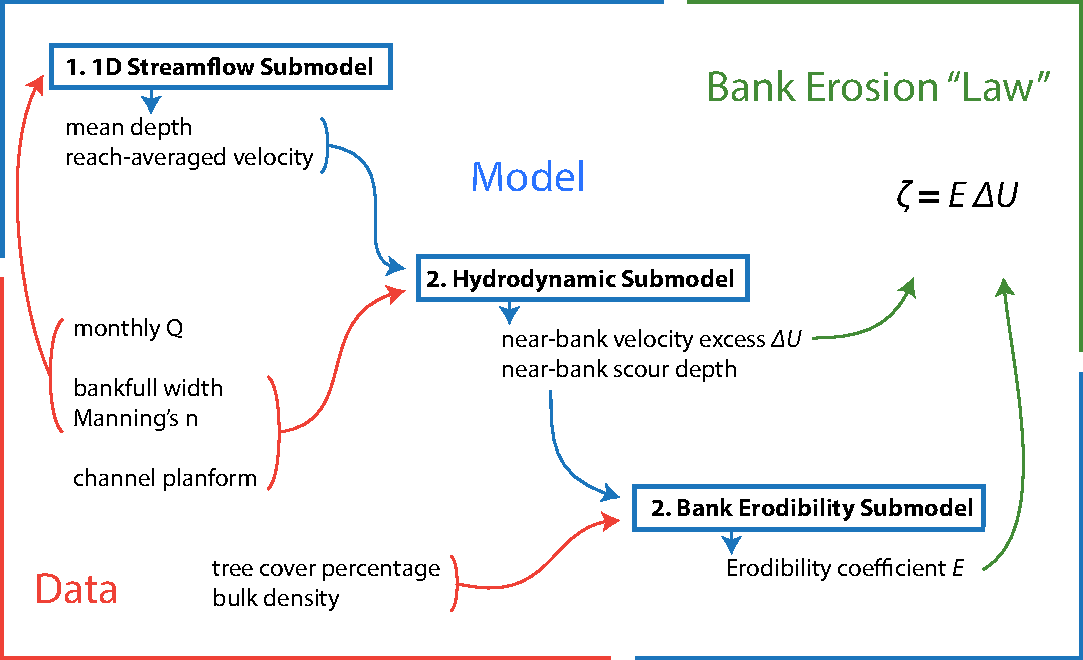
\includegraphics[width=1\textwidth]{figs/model-components.pdf}
\caption{Illustration of model data requirements (red), 3 main components (blue), and the geomorphic transport law used to model streambank erosion rate $\zeta$ (green).}\label{fig:model-components}
\end{figure}

In this paper, we test the hypothesis that a curvature-driven model of bank erosion, parameterized by remotely sensed data, can adequately represent point measurements of bank retreat at the outsides of bends over a large region after calibration by field observations obtained over a 2 yr period. The model of this paper quantifies annual streambank erosion rates by employing three interacting submodels: (1) a large-scale, 1-dimensional flow model of monthly discharge and steady uniform flow (streamflow submodel), (2) a physics-based hydrodynamic flow model (hydrodynamic submodel), and (3) a model of bank erodibility based on tree cover and bank height (bank erodibility submodel). These submodels, along with their assumptions and limitations are detailed below. \Cref{fig:model-components} gives a high-level overview of these components, their data requirements, and how they fit into the conceptual model (transport law) for bank erosion.

\section{Model components}

Streambank erosion rate $\hat{\zeta}$ (m/yr) was modeled as
\begin{equation}\label{eq:equation}
\hat{\zeta} = E \overline{\Delta U}
\end{equation}
where $\overline{\Delta U}$ (m/s) is the average near-bank velocity excess for a given simulation period, and $E$ is bank erodibility (here with units of s/yr). A large-scale 1-dimensional model for streamflow was coupled to a hydrodynamic model to estimate $\Delta U$. Two empirical, spatially distributed bank erodibility parameterizations of $E$ were investigated. For model calibration, simulation periods ranged from 22 to 24 mo for each location, depending on the dates of erosion rate measurements. \Cref{tab:inputs} summarizes the model input data. 

\begin{table}
\centering
\footnotesize
\begin{tabular}{rllll}
\toprule 
Model input & ~ & Units & Reference & Data source \\
\midrule
\multicolumn{5}{l}{\emph{Monthly time series}}\\
$^*$Streamflow & $Q_m$ & m$^3$/s  & \citet{Xia2012}& NLDAS-2, Noah-2.8 model \\
$^*$Storm frequency & $f_m$ & - & \citet{Rossi2015}& PRISM \\
$^*$Event discharge & $Q^*$ & m$^3$/s  & & $Q_m/f_m$  \\
$^*$Mean flow depth & $H$ & m & & Manning's equation\\
[3ex]
\multicolumn{5}{l}{\emph{Time-constant}}\\
$^*$Mean depth & $H_0$ & m & \citet{Metcalf2009} & Regional curves \\
$^*$Width & $B$ & m & \citet{Metcalf2009} & Regional curves \\
$^*$Friction factor & $C_\text{f,0}$ & - & \citet{George1989} & \Cref{tab:manning}\\
$^*$Channel slope& $S$ & m/m & & Extracted from DEM\\
$\dagger$Curvature & $R^{-1}$  & m$^{-1}$ & \citet{Guneralp2007}& USGS NED 3m\\
$\dagger$Tree cover & $\mathit{TC}$ & \% & \citet{Sexton2013} & USGS NED 3m \\
$\dagger$Bulk density & $\mathit{BD}$ & g/cm$^3$ & USGS Data Series 866  & SSURGO\\
Scour factor & $A$ & - & & Assumed const. = 3\\
\bottomrule
\multicolumn{5}{l}{$^*$Reach-averaged. $\dagger$Spatially variable at the reach scale.}\\
\multicolumn{5}{l}{NLDAS-2: National Land Data Assimilation Systems (\url{https://ldas.gsfc.nasa.gov/nldas/})}\\
\multicolumn{5}{l}{PRISM: PRISM Climate Group, Oregon State University (\url{http://prism.oregonstate.edu})}\\
\multicolumn{5}{l}{USGS NED 3m: National Elevation Dataset, 3 m per pixel (\url{https://datagateway.nrcs.usda.gov/})}\\
\multicolumn{5}{l}{GLCF: Global Land Cover Facility, The University of Maryland (\url{www.landcover.org}).}\\
\multicolumn{5}{l}{SSURGO: Soil Survey Geographic Database (USDA). (\url{https://dx.doi.org/10.3133/ds866})}\\
\bottomrule
\end{tabular}
\caption{Sources of data inputs for the streambank erosion model.}\label{tab:inputs}
\end{table}

\subsection{Monthly streamflow model}\label{sec:1d}
Rather than assuming mean annual discharge or bankfull discharge, a large-scale, 1-dimensional model for streamflow was included to account for spatial and temporal variability in runoff. This component was necessitated by the occurrence of sporadic high precipitation events in the study area, which seemed to be correlated to bank erosion events based on our field experience. The goal of the streamflow model is to estimate monthly flow depth $H_m$ and reach-average velocity $U$ for input into the hydrodynamic model. For $H_m$, Manning's equation can be written in terms of discharge as
\begin{equation}\label{eq:manningQ}
Q = \frac{1}{n}\frac{\displaystyle A_\text{c}^{5/3}}{\displaystyle P^{2/3}}S^{1/2}
\end{equation}
where $Q$ is water discharge (m$^3$/s) $A_\text{c}$ is cross-sectional area (m$^2$), $P$ is wetted perimeter (m), $S$ is longitudinal slope (m/m), and $n$ is Manning's roughness coefficient. Assuming a rectangular channel cross-section with flow of mean depth $H_\text{n}$ and width $B$, then $A_\text{c}=BH_\text{n}$ and $P=B+2H_\text{n}$. Substituting these expressions into \cref{eq:manningQ} yields
\begin{equation}\label{eq:manning}
Q = \frac{1}{n}\frac{\displaystyle\left(BH_\text{n}\right)^{5/3}}
{\displaystyle \left(B+2H_\text{n}\right)^{2/3}}S^{1/2}
\end{equation}
where, under the assumptions of steady uniform flow, $H_\text{n}$ (m) is the depth that corresponds to a given discharge, roughness, width, and slope: the so-called normal depth. \Cref{eq:manning} can be solved for $H_\text{n}$ using a variety of methods \citep{Vatankhah2013}. Here, \cref{eq:manning} was solved using Newton's method \citep{Tiwari2012}. Monthly discharge was provided by the Noah-2.8 land surface model described below \citep{Sexton2013}. For each month, reach average velocity (m/s) was calculated as
\begin{equation}
U = Q*/(BH_\text{n})
\end{equation}
where $Q*$ represents an estimate of the average monthly discharge during high flow events. Although the use of a 1-dimensional model is necessarily simplified, the hydrodynamic model only requires estimates of 1-dimensional flow variables, reach-averaged velocity $U$ and flow depth $H_\text{n}$.

\subsection{Hydrodynamic model}\label{sec:bdv}
The hydrodynamic model component drives streambank erosion by providing the near-bank velocity excess $\Delta U$ (\cref{eq:ikeda}). The hydrodynamic model developed by Blanckaert and de Vriend (\citeyear{Blanckaert2003}, \citeyear{Blanckaert2010}) was chosen because, unlike other reduced-order models, it does not assume mild curvature or weak curvature variations \citep{Ottevanger2012}. Because hydrodynamic models built on mild-curvature assumptions can overestimate the effects of secondary flow in sharp bends \citep{Ottevanger2012}, the model of \citet{Blanckaert2010} was considered more appropriate for the study area, where sharp bends are common (\cref{fig:centerlines}). Source code for this model has been provided by \citet{Ottevanger2013} through the OpenEarth repository (\url{https://publicwiki.deltares.nl/display/OET/OpenEarth}).

In the hydrodynamic model of \citet{Blanckaert2010}, hereafter referred to as the BdV model, the downstream velocity width-distribution, which leads to near-bank velocity perturbations, is parameterized by $\alpha_\text{s}/R$, where $\alpha_\text{s}=-1$ corresponds to a potential vortex distribution and $\alpha_\text{s}=1$ to a forced vortex distribution. In straight reaches, $\alpha_\text{s}$ is near zero and near-bank velocity is close to the average velocity \citep{Blanckaert2003}. The streamwise development of $\alpha_\text{s}/R$ is represented by a relaxation equation. The relaxation equation has an adaptation length largely controlled by $C_\text{f}^{-1} H/R$, and driving mechanisms representing transverse slope, curvature forcing, secondary flow, and velocity redistribution by the secondary flow \citep[][equations 35--37]{Blanckaert2010}. Near-bank depth excess $\Delta h$ (m) is induced by basal scour and is given by $\Delta h=HA/R$, where the $A/R$ term parameterizes transverse bed slope. The streamwise development of $A/R$ is represented by a relaxation equation with an adaptation length dependent on $H$ and $C_\text{f}$ \citep[][equation 20]{Blanckaert2010}. 

Natural rivers show variability in the scour factor $A$, but a typical range of 2.5 to 6 is often cited (e.g., \citealp{Ikeda1981}; \citealp{Ottevanger2012}), or $A$ is treated as a calibration parameter \citep{Odgaard1987}. In this model, $A$ was assumed a constant value of 3. Although our field data do not allow characterization of $A$ throughout each reach, the average value of $A$ measured from individual cross-sections was 2.9, which supports our estimated constant value of $3$. Modeled bed topography was initialized before beginning the simulations by setting $A=3$ and allowing $A/R$ to adjust to bankfull flow conditions. $A$ was then kept constant throughout monthly simulations. Assuming a constant $A$ is a limitation of this implementation, which is designed to be applicable at the reach and watershed scale by using remotely-sensed data. If this is not a requirement, spatial variations in $A$ can be measured in the field.

The near-bank values of $\Delta U$ (m/s) and $\Delta h$ (m) were obtained throughout each reach by the following equations
\begin{align}
\Delta U &= U_\text{s}\frac{\alpha_\text{s}}{R}\frac{B}{2}\\[0.5em]
\Delta h &= H\frac{A}{R}\frac{B}{2}
\end{align}
where $U_\text{s}$ is the reach-averaged velocity (m/s) and $H$ is the cross-sectional average flow depth (m) given by the 1-dimensional streamflow model (\cref{sec:1d}). Bank height was modeled as the bankfull mean depth plus the near-bank depth excess due to basal scour, $H_\text{b} = H_{0} + \Delta h$. This height corresponds to the underwater portion of the bank in the BdV model and does not account for floodplain elevation. Natural streams are thus likely to have higher banks than $H_\text{b}$ predicts. A more accurate estimate of bank height could be made by adding $H_\text{b}$ to bank heights extracted from a high resolution digital elevation model, which would represent the subaerial portion of the banks. The data currently available do not permit this for the studied reaches. As a consequence, the bank heights of most studied reaches are under-predicted by the current model.

The BdV model assumes a linear transverse velocity profile that is equal to the reach-averaged velocity at the channel centerline. Therefore, only one bank has a positive velocity perturbation $\Delta U$, while the opposite bank has an equally strong negative velocity perturbation. Meander migration models based on \cref{eq:ikeda} have usually assumed that channel width remains constant over the simulation period \citep{Parker2011}, and thus that deposition occurs on the opposite bank to keep pace with the eroding bank. The model of this paper is concerned with monthly to annual erosion rates, and not with long-term channel evolution and meander migration. Therefore, it does not make any assumptions about the accretion of the opposite bank. Instead, $\Delta U$ is set to zero at locations where it is modeled to be negative. As a consequence of this set of assumptions, erosion is only allowed to occur where $\Delta U > 0$ and it is restricted to only one side of a given cross-section. This is a limitation of many meander morphology models, including the present one. It is worth noting, however, that the eroding bank does not necessarily correspond to the concave bank in this model; due to the BdV model's nonlinear parameterization of the flowfield and the spatial lag between curvature and velocity perturbations, the convex bank may host positive $\Delta U$ values, especially in tight bends. The BdV model was run on a monthly timestep by varying the monthly event discharge and flow depth according to the procedure detailed above. Prior to the initial model simulation of each channel, bankfull discharge and flow depth conditions were simulated to set the initial bed geometry, and this geometry was held constant throughout subsequent monthly simulations.

\subsection{Bank erodibility parameterization}

The bank erodibility coefficient $E$ of \cref{eq:equation} was assumed to be proportional to soil erodibility, here denoted $K$. Two representations of soil erodibility, $K_1$ and $K_2$, were investigated. \citet{Wynn2006} provided an empirical equation for sandy streambank soils in southwestern Virginia expressed as a function of coarse root density and soil bulk density at the bank toe,
\begin{equation}\label{eq:wynn}
K_1 = c_0\exp \left(c_1\ln\mathit{RD} - c_2\mathit{BD}^{2.5}\right)
\end{equation}
where $\mathit{RD}$ is root density, defined as the volume of coarse roots (2--20~mm in diameter) per volume of soil (cm$^3$/cm$^3$), $\mathit{BD}$ is soil bulk density (g/cm$^3$), and $K_1$ is soil erodibility with units of cm/N/s \citep{Wynn2006}. Due to the normalization and empirical fitting of the original data by \citet{Wynn2006}, we replaced the coefficients with generic calibration constants, $c_0$, $c_1$, and $c_2$; the exponent of 2.5 was retained. \citet{Pizzuto1984} and \citet{Pizzuto1989} found that for forested streambanks, bank erodibility was not related to soil properties but was largely controlled by vegetation density. Therefore, the second representation of soil erodibility was a power function of root density $\mathit{RD}$,
\begin{equation}\label{eq:k2}
K_2 = c_3 \mathit{RD}^{c_4},
\end{equation}
where root density is defined as the total volume of roots per volume of soil (cm$^3$/cm$^3$), and $c_3$ and $c_4$ are calibration constants. In both $K_1$ and $K_2$, $\mathit{RD}$ was estimated as a function of tree cover and bank height. Because root distributions decrease exponentially with depth below the ground surface \citep{Zeng2001}, $\mathit{RD}$ at the bank toe was modeled as a function of tree cover and bank height,
\begin{equation}\label{eq:rd}
\mathit{RD} = c_5\mathit{TC}^{c_6} \exp(c_7 H_\text{b})
\end{equation}
where $\mathit{TC}$ is tree cover (the fraction of ground area covered by vegetation $>$5m tall), $H_\text{b}$ is bank height (m), and $c_5$, $c_6$, and $c_7$ are calibration constants. \Cref{eq:rd} assumes that all trees are growing on a flat floodplain area adjacent to the bank, and not on the bank itself, and thus underestimates the effects of trees growing directly on the bank. Two model formulas were fitted separately, one assuming $E=K_1$, and another assuming $E=K_2$ \cref{tab:model-eqns}. After combining calibration constants as appropriate, these models contain 4 and 3 free parameters, respectively. The following sections detail the implementation of this model and present the results of calibrating the model using streambank erosion rates measured over a period of 2.5 yr in the northern Gulf of Mexico coastal plain.

\begin{table}
\centering
\begin{tabular}{lll}
\toprule 
Model formula & Bank erodibility & Free parameters* \\
\midrule
$\hat{\zeta}_{1} = a_0 \exp\left(a_1 \ln(\mathit{TC}) + a_2 H_\text{b} + a_3 \mathit{BD}^{2.5} \right)\overline{\Delta U}$ & $K_1$ (\cref{eq:wynn}) & $a_0$, $a_1$, $a_2$, $a_3$\\
 $\hat{\zeta}_{2} = b_0 \mathit{TC}^{b_1}\exp(b_2 H_\text{b})\overline{\Delta U}$ & $K_2$ (\cref{eq:k2}) & $b_0$, $b_1$, $b_2$\\
 \midrule
 \multicolumn{3}{l}{*$a_0=c_0\exp(c_1\ln c_5)$, $a_1=c_1 c_6$, $a_2=c_1 c_7$, $a_3=c_2$} \\
 \multicolumn{3}{l}{*$b_0=c_0 c_3 c_5$, $b_1=c_3 c_4$, $b_2=c_7 c_4$} \\
\bottomrule
\end{tabular}
\caption{Two model formulas fitted in this paper. The models differ by their parameterization of soil erodibility and number of free parameters. $\hat\zeta$: Modeled streambank erosion rate (m/yr). $\mathit{TC}$: Tree cover fraction. $H_\text{b}$: Modeled bank height (m). $\mathit{BD}$: Soil bulk density (g/cm$^3$). $\overline{\Delta U}$: Average near-bank velocity excess (m/s).}\label{tab:model-eqns}
\end{table}

\section{Data sources and processing}

\subsection{Streambank erosion calibration database}

Streambank erosion rates were measured during the 2014, 2015, and 2016 water-years at 30 streambank locations throughout the northern Gulf of Mexico coastal plain (\cref{fig:sites}). The study locations were selected to represent variability in channel size, geometry, and vegetation density. All channels included in this study are single-thread, meandering, sand-bed channels, the dominant channel type in the study area \citep{Metcalf2009}. A majority of studied channels (20) were Rosgen type E, which corresponds to sinuous channels with low width-to-depth ratios generally $<$12 \citep{Rosgen1994}. Rosgen type C streams were also common (7 sites), while type F (2 sites) and type G (1 site) streams, which correspond to incised channels, were relatively rare. \Citet{Metcalf2009} also identified predominately type C and E streams in the study area. Only wadeable streams were studied. Drainage areas were relatively small, most being $<$100 km$^2$. Streambank characteristics measured in the field are summarized in \cref{fig:boxplots}.

\begin{figure}
\centering
\frame{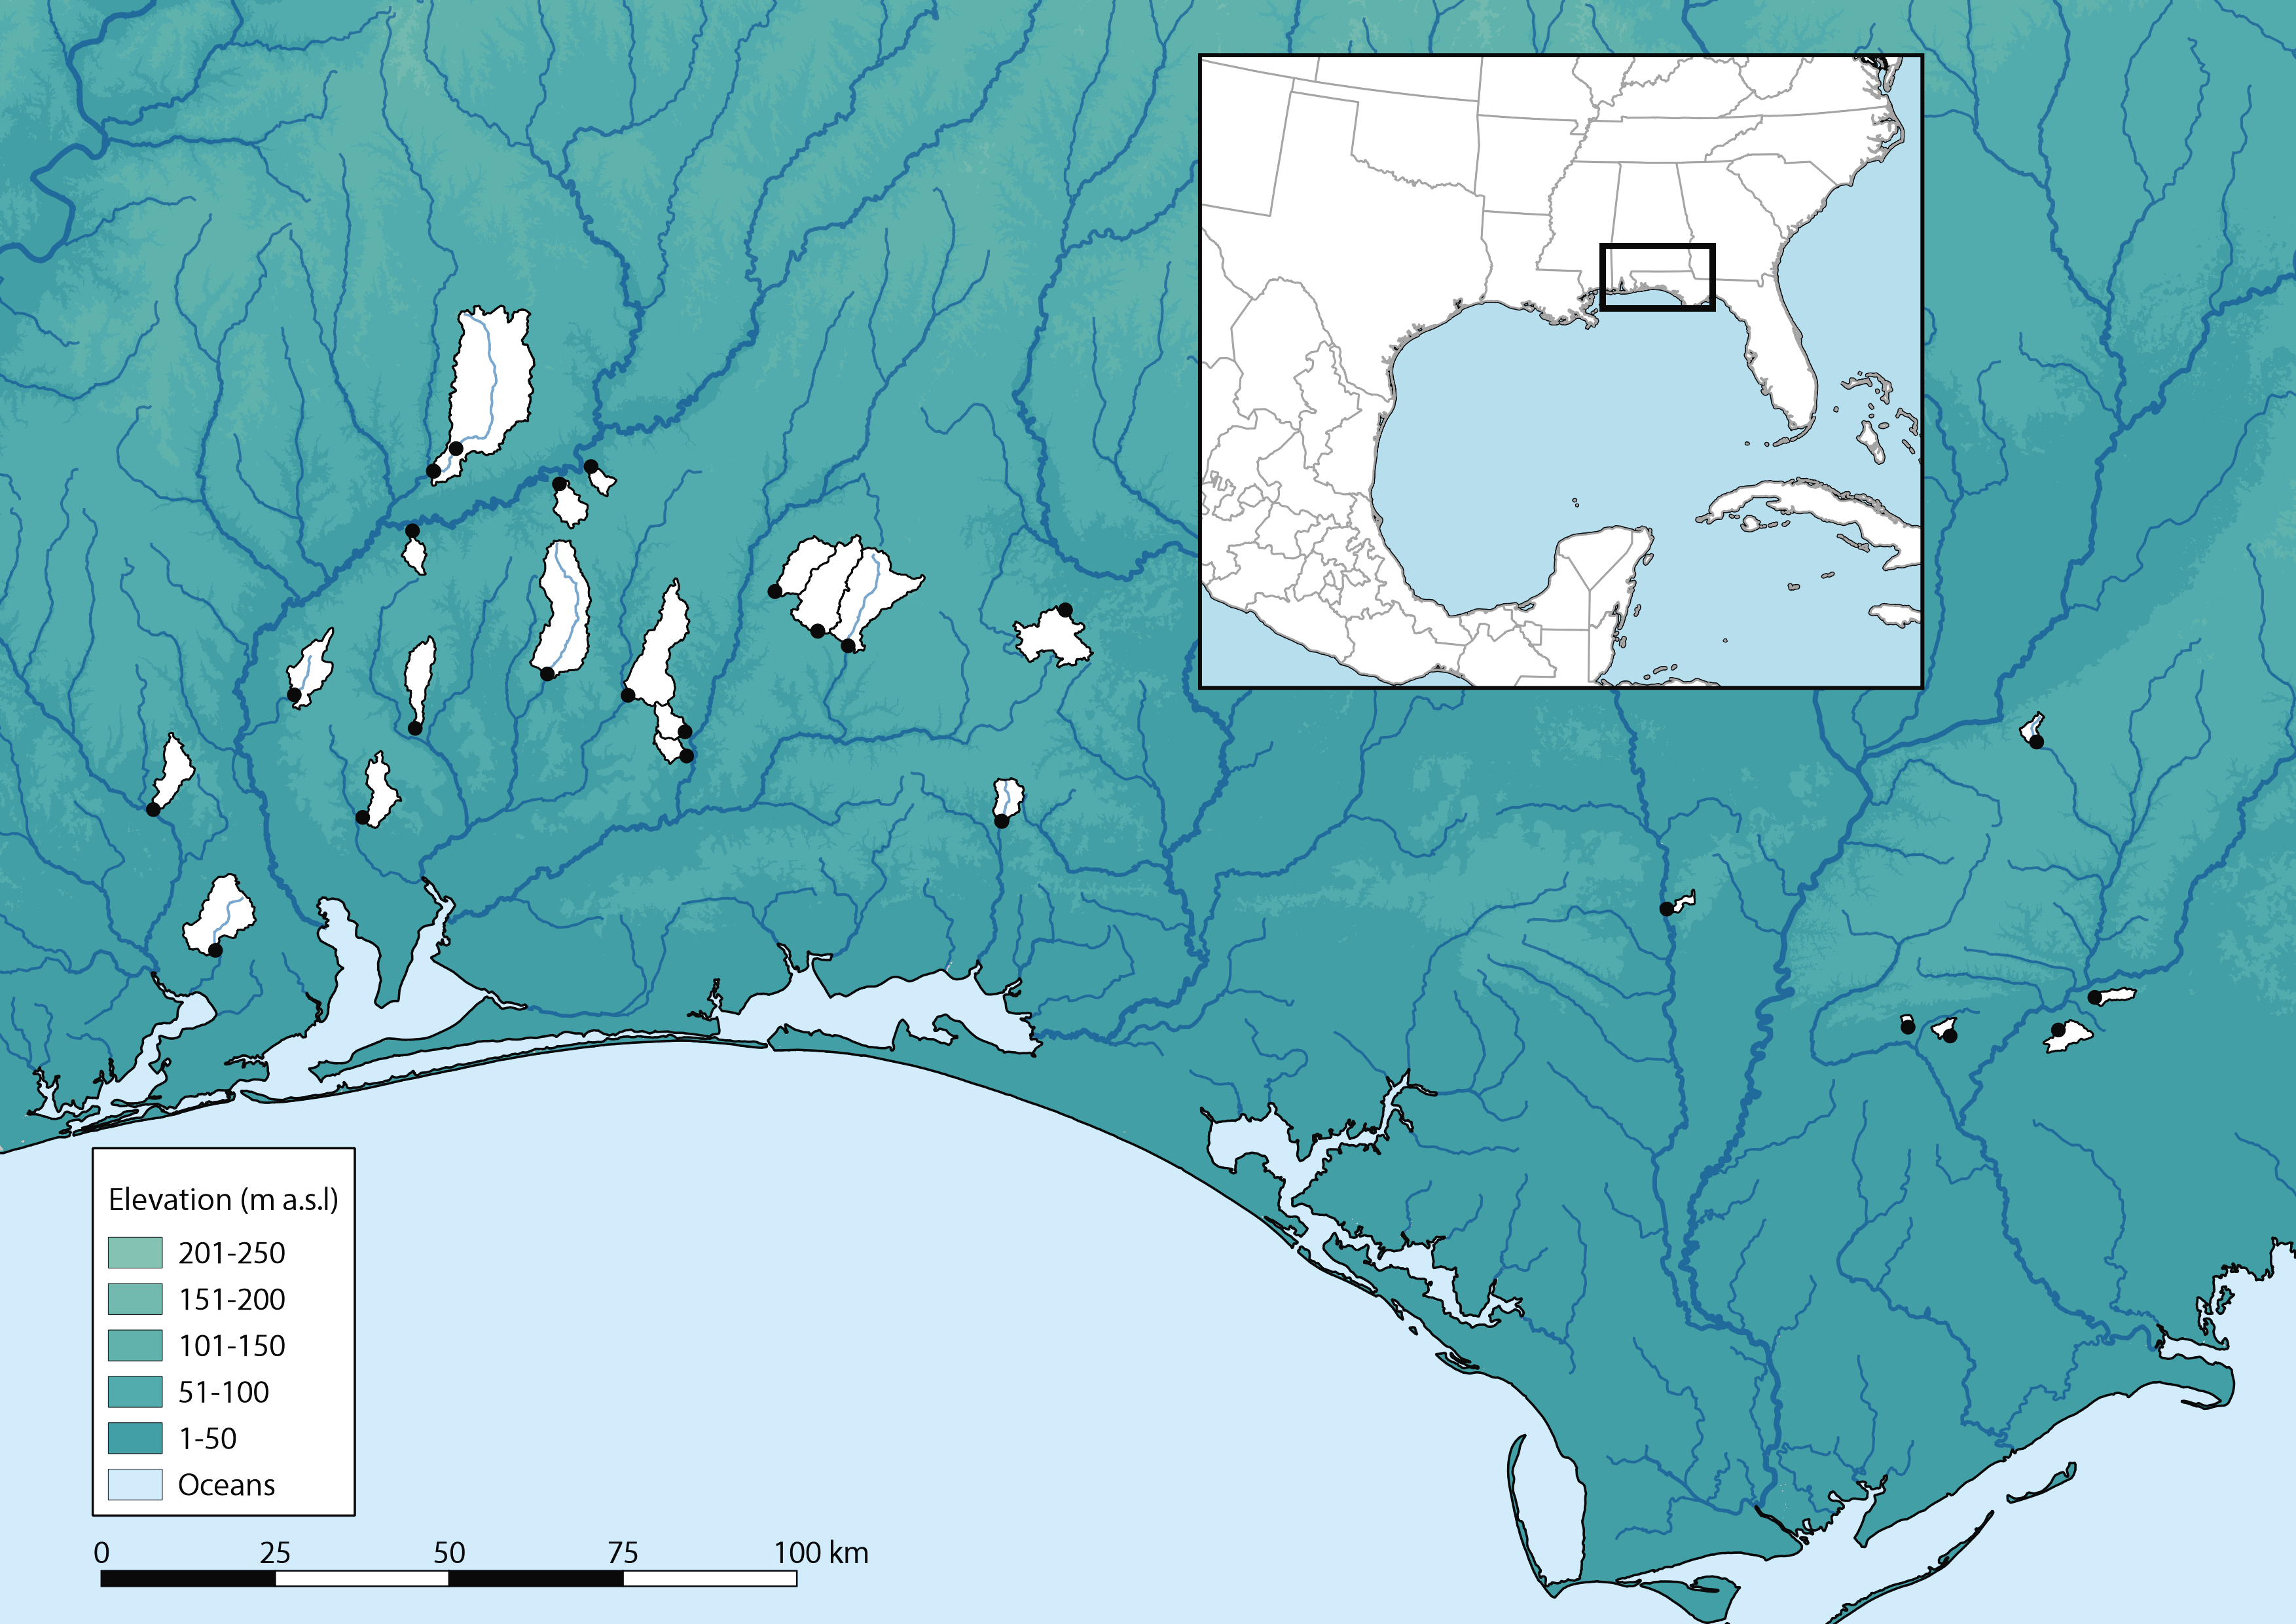
\includegraphics[width=1\textwidth]{figs/study-area-model.png}}
\caption{Elevation map showing locations of measured streambank erosion rates (black circles) and their corresponding watershed areas (white). Inset map: Location of the study area within the northern Gulf of Mexico coastal plain.}\label{fig:sites}
\end{figure}

Streambank erosion was monitored using repeated cross-profiling, which involved measuring the distance to the bank from a rebar pin placed at the bank toe \citep{Lawler1993}. Measurements were taken at vertical intervals of 5--50 cm, depending on bank height, and at major breaks in slope \citep{Bangen2014}. Vertical profiles were measured once per year, resulting in final streambank erosion rates averaged over approximately two years for each location. In addition to the vertical profile sections, full channel cross-sections were measured during the initial and final site visits, and were used to determine channel geometry.

\begin{figure}
\centering
\frame{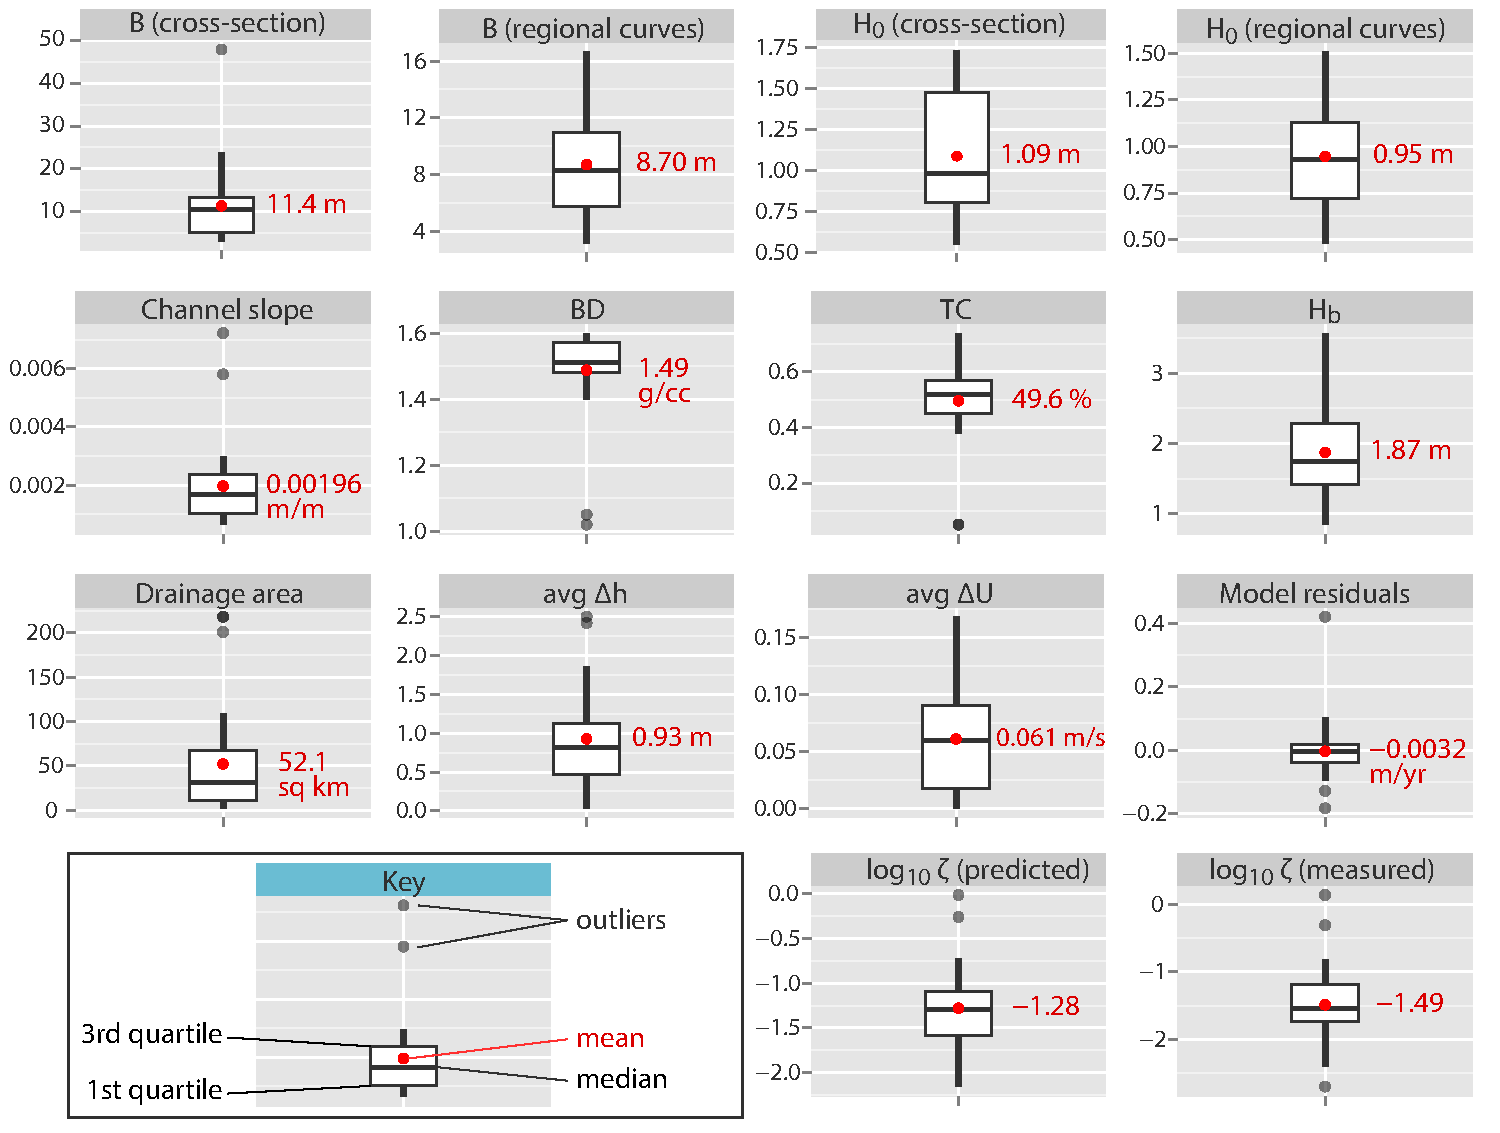
\includegraphics[width=1\textwidth]{figs/model-boxplots.pdf}}
\caption{Box-and-whisker plots of field measured data, model inputs, model predictions, and residuals. The whiskers extend to the largest (or smallest) observations that are within 1.5 times the interquartile range of the boxes. Outliers are data points that lie outside of the range of the whiskers. Average values refer to the average of the monthly time series at each study site. Erosion rate statistics do not include values less than or equal to zero.}\label{fig:boxplots}
\end{figure}

Erosion rates ranged from 0--1.38 m/yr and were heavily right-skewed, with a mean of 0.094 m/yr, median of 0.027 m/yr, and standard deviation of 0.26 m/yr (\cref{fig:hist}). A majority of the studied streambanks (21) had low erosion rates, $<$0.05 m/yr, including three with no measurable erosion or slight deposition.  Because this paper models erosion processes and not deposition, locations that had negative erosion rates ($n=4$) were assigned values of zero and included in the modelling. Two streambanks retreated at rates greater than 0.4 m/yr; these outliers are apparent in the histogram in \cref{fig:hist} and even on the log-transformed data in \cref{fig:boxplots}. Erosion rates were thus low on average but highly variable. 

Because the model was designed to utilize widely available remote sensing data, rather than field data collection, no other field measurements were incorporated into model. Bankfull channel widths and depths measured at single cross-sections are included in \cref{fig:boxplots} for comparison to the modeled values of width and depth obtained through regional curves as described below.

\begin{figure}
\centering
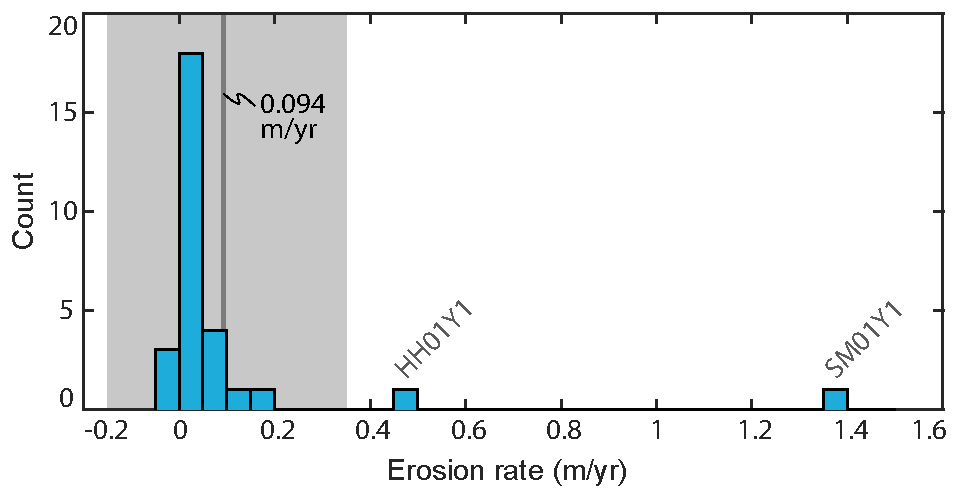
\includegraphics[width=0.8\textwidth]{figs/model-erosion-hist.pdf}
\caption{Histogram of measured erosion rates, averaged over 2 yr, including those less than or equal to zero. Bin widths are equal to 0.05 m/yr. The mean (0.094 m/yr) is shown as the thick gray line. The shaded area represents 1 standard deviation (0.26 m/yr) on either side of the mean. Two outliers are labeled with identifiers that correspond to their rows in the supplementary data table.}\label{fig:hist}
\end{figure}

\subsection{Channel geometry data}

Bankfull channel width $B$~(m) and bankfull mean depth $H_0$~(m) were estimated using regional curves developed by \citet{Metcalf2009}. Regional curves predict bankfull channel geometry from drainage area. Similar equations are available in many regions of the United States (\citealp{Faustini2009}; \citealp{Bieger2015}). In the U.S., the Natural Resources Conservation Service maintains a database of regional curve studies organized by physiographic province (NRCS, Regional Hydraulic Geometry Curves, \url{http://www.nrcs.usda.gov/wps/portal/nrcs/detail/national/water/?cid=nrcs143_015052}). If regional curves are unavailable, channel geometry can be estimated with other methods or measured in the field. For a given reach, $B$ was held constant throughout all model simulations and $H_0$ was only used to set the initial bed geometry. Spatial and temporal variation in flow depth were modeled explicitly (\cref{sec:bdv}).

Drainage areas were extracted from the National Hydrography Dataset (NHD) Plus v2 using the NHD Plus v2 Basin Delineator Tool. Due to heavy tree cover, channel centerlines were digitized on USGS 3D Elevation Program (3DEP) DEM (horizontal resolution 1--3 m. In less heavily-forested areas, channel centerlines can be accurately digitized using aerial or satellite imagery (\citealp{Guneralp2007}; \citealp{Guneralp2013}; \citealp{Guneralp2014}). 

Digitized centerlines were interpolated with parametric piecewise-cubic spline (PCS) functions $X(s)$ and $Y(s)$, where $s$ is downstream distance (m), and curvature was calculated analytically as 
\begin{equation}
\frac{1}{R} = \frac{\displaystyle X'Y'' - Y'X''}{\displaystyle \left[(X')^{2} + (Y')^{2}\right]^{3/2}}
\end{equation}
where $R$ is radius of curvature (m) \citep{Guneralp2007}. The downstream coordinate $s$, curvature $1/R$, and unit normal vectors $n$ were discretized at intervals of $B/10$ meters. \Cref{fig:centerlines} plots these interpolated channel centerlines, which were ultimately used to train the model. Channel gradients were estimated by extracting a topographic profile along the channel centerline and robust weighted linear regression fitting. For four reaches (five individual sites) that were not resolved by the 3DEP DEM due to especially dense vegetation cover, a 50 cm DEM was created from terrestrial laser scanning (TLS) data collected during the study period. These reaches included Willacoochee Creek (sites WC01 and WC02; \cref{fig:tls}), Blue Creek (site OR01) Grab Mill Creek (site GM01), and Hollis Branch (site CH01). TLS DEMs were obtained data by taking the minimum height of each 50 cm grid cell (\cref{fig:tls}).

\begin{figure}
\centering
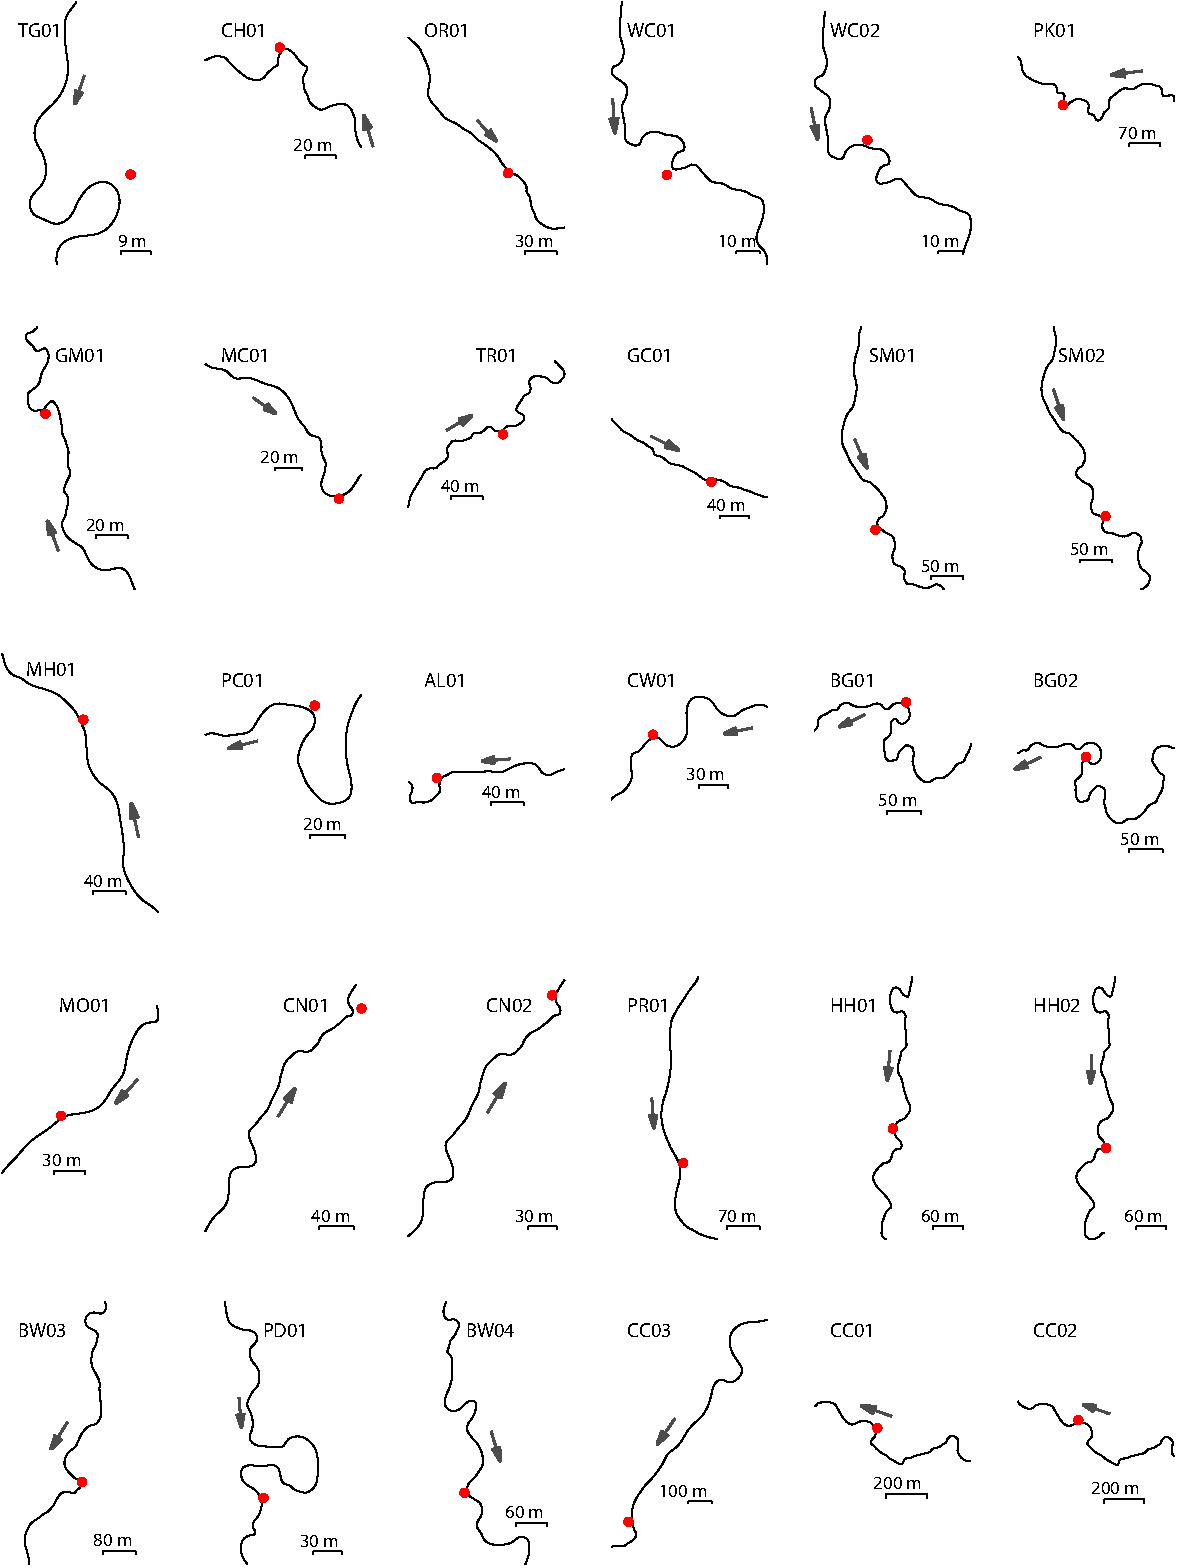
\includegraphics[width=0.9\textwidth]{figs/centerlines.pdf}
\caption{Illustration of channel centerlines derived from piecewise-cubic spline interpolation. Red dots show the locations of streambank erosion monitoring sites. Arrows indicate the general flow direction.}\label{fig:centerlines}
\end{figure}

\begin{figure}
\centering
\frame{\includegraphics[width=1\textwidth]{figs/wc01-tls.png}}
\caption{Example DEM created from TLS data collected during the study period overlaid on a DEM of the highest-available resolution at the time of writing (10 m National Elevation Dataset) showing two streambank erosion monitoring sites (WC01, WC02) and the digitized channel centerline (black polyline with arrows indicating flow direction). The upper right inset shows the channel profile extracted from this reach (blue dots), and the robust linear regression line used to estimate channel slope (black line) with 80x vertical exaggeration. Willacoochee Creek, SW Georgia.}\label{fig:tls}
\end{figure}

\subsection{Monthly streamflow data}
The Noah-2.8 land surface model (LSM) with National Land Data Assimilation Systems Phase 2 (NLDAS-2) forcings (\citealp{Mitchell2004}; \citealp{Xia2012}) allowed calculation of the average monthly discharge,  $Q_m$ (m$^3$/s), from each drainage basin. These data are available in $1/8^{\circ}$ grid cells representing average values within each cell. This scale is similar in size to many of the watersheds in this study. Due to the coarse resolution, a pre-processing step was applied of cubic convolution downscaling to $\sim$100 m. $Q_m$ was computed as the sum of basin-accumulated baseflow and surface runoff during each month.

Streamflow was simulated for each month by assuming a monthly event discharge, i.e., the average discharge through the channel during periods of high flow events. We assume that this event discharge is more relevant for bank erosion than average monthly or average annual discharge, which tend to be significantly lower due to long periods of baseflow. A simple method was devised to quantify the event discharge $Q^*_m$ for each month $m$ as $Q^*_{m}=Q_m/f_m$, where $Q_m$ (m/s) is average monthly discharge, and $f_m$ is monthly storm frequency (dimensionless). Average monthly storm frequency was calculated from daily gridded precipitation rasters from the PRISM Climate Group (\url{www.prism.oregonstate.edu}) as the ratio of wet days ($>$1 mm precipitation) to total days in each month \citep{Rossi2015}. Note that as storm frequency approaches one, $Q^*_m$ approaches the average monthly discharge, and as storm frequency decreases toward zero, $Q^*_m$ increases relative to $Q$. This reflects the strong effects that large, infrequent storms may have on streamflow. $Q^*_m$ was assigned to zero for months with $f_m = 0$, though this did not occur during the study period.

\subsection{Channel friction}

Dimensionless channel friction is defined as the square of the shear velocity divided by average velocity,
\begin{equation}\label{eq:cf}
C_\text{f} = \left(\frac{u_*}{U_\text{s}}\right)^2
\end{equation}
where $u_*=\sqrt{\tau / \rho}$ is the shear velocity (m/s), $\tau$ is average boundary shear stress (Pa), and $\rho$ is the density of water (kg/m$^3$). The hydrodynamic model described below requires the dimensionless friction factor for a theoretical straight channel, $C_\text{f,0}$, and the extra drag induced by meandering is simulated by the hydrodynamic model itself. Therefore, \cref{eq:cf} is written in terms of Manning's roughness coefficient $n$,
\begin{equation}\label{eq:cf0}
C_\text{f,0} = \frac{\displaystyle g R_\text{h} S}{\displaystyle U_\text{s}^2} = g\left(\frac{\displaystyle n}{\displaystyle R_\text{h}^{1/6}}\right)^2
\end{equation}
which allows straight channel roughness to be calculated by assuming a constant $n$. The hydrodynamic model assumes a trapezoidal channel cross-section (rectangular in straight reaches), which allows the hydraulic radius $R_\text{h}$ to be calculated as $BH_0/(B+2H_0)$.

\Citet{Sefick2015} report that $n$ can be estimated using three general approaches: consulting a table relating $n$ to qualitative channel characteristics, comparing studied channels to photographs of channels where $n$ has been measured, or using empirical relationships based on hydraulic variables. The difficulties in empirically estimating $n$ have been well documented, especially for sand bed channels, where the roughness associated with bedforms changes with discharge \citep{Ferguson2010}. It is also difficult to account for the large roughness elements introduced by dense vegetation using empirical relationships based on grain size and other bed parameters. As an alternative, semi-quantitative approach, $n$ can be estimated as the sum of five components times a sinuosity factor $m$,
\begin{equation}\label{eq:n}
n = m(n_\text{b} + n_1 + n_2 + n_3 + n_4)
\end{equation}
where $n_\text{b}$ is a base coefficient for a given boundary material, and $m$ ranges from 1 to 1.3 to account for the increased drag of meandering channels \citep{George1989}. \Cref{tab:manning} gives estimates for $n_\text{b}$ and $n_1$ through $n_4$ used in this study. For $n_b$, a base value representing bed material roughness, we assumed a median grain diameter of 0.2 mm, corresponding to fine sand, based on our qualitative observations of grain size during field work. The other components, which are semi-quantitative, are also estimated based on field experience. This results in a characteristic value of $n=0.087$ for a straight channel (letting $m=1$). This value was assumed constant throughout the study area and corresponds to $C_\text{f,0}$ values around 0.05--0.11, which are significantly larger than the values for rivers reported by \citep{Ottevanger2012}, but representative of the sharp, narrow, highly vegetated channels in the study area \citep{Thorne1995}. \Cref{eq:n} assumes that $n$ is constant for all discharges, does not account for bedform drag, and is based on semi-quantitative estimations of vegetation density, surface irregularity, and channel obstruction, and thus amounts to an order of magnitude estimate.

\begin{table}
\centering
\begin{tabular}{lll}
\toprule
Component & Modeled value & Meaning\\
\midrule
$n_b$ & 0.012 & Sand bed with $D_{50} \sim 0.2$ mm\\
$n_1$ & 0.01 & Moderate--severe surface irregularity\\
$n_2$ & 0.015& Frequently alternating cross-section\\
$n_3$ & 0.02 & Minor obstruction ($<15\%$ channel area)\\
$n_4$ & 0.03 & Large amount of vegetation\\
$m$ & 1.0 & Sinuosity $=1$ (for BdV model)\\
\midrule
$n$ & 0.087 & Manning's $n$ in this model\\
\bottomrule
\end{tabular}
\caption{Values used to calculate Manning's $n$ for a theoretical straight channel. $D_{50}$ is median grain diameter. BdV: \citet{Blanckaert2010}.}\label{tab:manning}
\end{table}

\subsection{Soil erodibility data}
Soil erodibility was modeled using $K_1$ (\cref{eq:wynn}) and $K_2$ (\cref{eq:k2}). Area- and depth-weighted average bulk density was obtained from the SSURGO dataset in the form of a 10 m raster (Wieczorek, M. E., USGS Data Series 866, \url{http://water.usgs.gov/GIS/metadata/usgswrd/XML/ds866_ssurgo_variables.xml}). 

Root density $\textit{RD}$ was modeled as a function of tree cover $\mathit{TC}$ and bank height $H_b$ (\cref{eq:rd}). Tree cover was obtained as a 30 m raster from the Global Land Cover Facility at the University of Maryland, which represents the fraction of each 900 m$^2$ pixel covered by vegetation greater than 5 m in height \citep{Sexton2013}. This dataset is based on Landsat observations, is free to the public, covers the entire globe, and is readily available online (\url{http://www.landcover.org/data/landsatTreecover/}). Three datasets are available based on observations from 2000, 2005, and 2010. Although erosion rates were measured during 2014--2016, the 2010 dataset contains many small gaps associated with cloud cover. Therefore, the 2005 dataset was used. Although the 2005 tree cover dataset is approximately 10 yr out of date, it is highly unlikely that any of the small headwater streams investigated in this study have shifted significantly at the 30 m/pixel scale since 2005. The largest erosion rate observed in this study, $\sim$1.3 m/yr, corresponds to a total lateral shift of 13 m over 10 yr, assuming that such a high erosion rate is sustained over the 10 yr period. Additionally, no major forest disturbances were observed at any of the study sites, which would be obvious had they occurred during the last 10 yr in the study area. Most studied streambanks hosted trees of varying species and diameters, which qualitatively supports the moderately high values of tree cover exhibited in the 2005 dataset. Most sites hosted trees greater than 30 cm in diameter, which indicates that they have been growing for much longer than 10 yr. One exception is Sconnier's Mill Creek (sites SM01 and SM02), which has recently lost much of its tree cover in a limited area near the bank. Based on our field experience, an estimated value of 5\% was assigned as input for this location. All other locations used values from the 2005 tree cover dataset. If this model is applied in more dynamic environments in the future, the 2005 tree cover dataset may prove to be inadequate, in which case the 2010 dataset may be used, or tree cover may be estimated using different methods.

\subsection{GIS environment}
The raster data representing tree cover, bulk density, and monthly streamflow and the polylines representing channel geometry were managed in a geographic information system (GIS) using Matlab (\cref{fig:setup}). The 30 m pixel size of these raster data is relatively coarse compared to the studied channel reaches. Errors can arise if the raster data are sampled at pixels representative of the opposite streambank or corresponding to the mid-channel open water. Therefore, rasters were sampled at bank locations, rather than channel centerlines. Left- and right-bank locations were modeled as one channel width from each centerline using the unit normal vectors $n$ calculated during PCS-interpolation of the channel centerline. To associate measured erosion rates to a modeled bank location and channel centerline node, the GPS locations recorded in the field were matched with the nearest-neighbor bank location (\cref{fig:setup}).

Rasters were sampled at runtime by looping through the bank point locations and extracting (Matlab function \emph{imread}) and interpolating the four nearest pixels from the raster dataset. This approach has the advantage that rasters of differing resolution and/or spatial references can be used without the need to reproject the entire raster, provided that geotransforms exist between the various spatial reference coordinates. This allows entire river reaches to be modeled efficiently. Bilinear interpolation results in bank erodibility estimates that vary smoothly throughout a meander bend, rather than in sharp jumps characteristic of the raw raster pixels. Each bank location, therefore, is assigned unique values of tree cover and bulk density as well as a value of near-bank velocity excess and bank height from the hydrodynamic model.

\begin{figure}
\centering
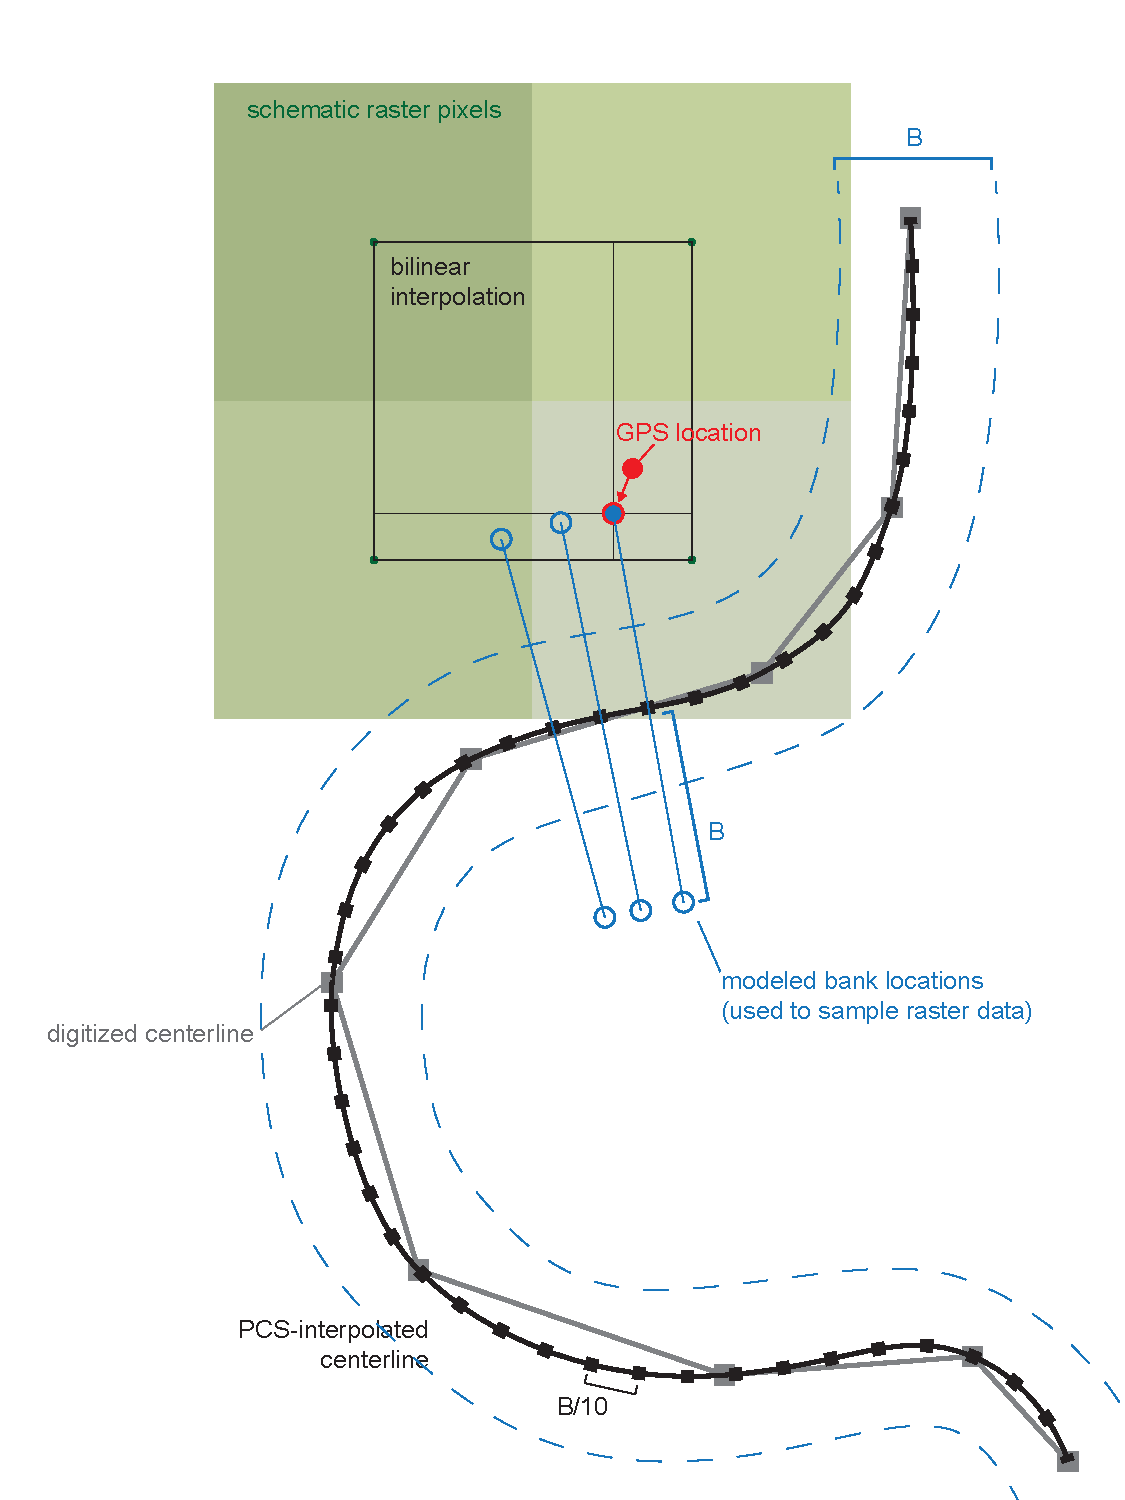
\includegraphics[width=0.9\textwidth]{figs/model-setup.pdf}
\caption{GIS environment. Centerlines digitized on a 3 m DEM (gray polyline) were PCS-interpolated (black). Banks locations (blue circles) were assumed $B$ meters (channel width) from the centerline. The bank point nearest the cross-section as surveyed in the field (red circle) was selected. The 4 nearest raster pixels were interpolated (green squares).}\label{fig:setup}
\end{figure}

\subsection{Regression analysis}\label{sec:regression}
Given the model structure presented above and the model formulas of \cref{tab:model-eqns}, the free parameters must be estimated by minimizing model error. There are at least three straightforward options, however, each with its own set of assumptions regarding error structure. Letting $f(x)$ represent an arbitrary, nonlinear function of independent variables, erosion rate $\zeta$ can be modeled as

\begin{align}
\zeta &= f(x) + \epsilon \label{eq:constant} \\
\zeta &= f(x) \cdot \epsilon \label{eq:proportional} \\
\zeta &= f(x) \cdot \exp(\epsilon) \label{eq:exponential}
\end{align}
where $\epsilon$ is normal error, $\epsilon \sim \mathcal{N}(0, \sigma)$. \Cref{eq:constant} assumes that error is additive and normally distributed, \cref{eq:proportional} assumes that error is multiplicative and normally distributed, and \cref{eq:exponential} assumes that error is multiplicative and lognormally distributed \citep{Xiao2011}. It is worth noting that \cref{eq:exponential} results from log-transforming both sides of a nonlinear equation, e.g., a power-law relationship, which is commonly done to linearize the equation for practical or scientific reasons \citep{Xiao2011}. The choice of error model can often have a large impact on the final values of regression parameters and thus also on the conclusions drawn from modelling studies.

We investigated all three error models while calibrating the free parameters. Normal additive and normal multiplicative error models were investigated through nonlinear regression (Matlab function \emph{fitnlm}); lognormal multiplicative error was investigated by log-transforming the data for the equations given in \cref{tab:model-eqns} and linear regression of the log-transformed data. Only the normal multiplicative error model (\cref{eq:proportional}) resulted in accurate predictions of streambank erosion rate. Additionally, for stochastic events such as streambank erosion, variance is proportional to the maximum magnitude of individual events \citep{Pizzuto2010}, which we interpret as further evidence that a regression model with proportional error variance is most appropriate.

In the context of nonlinear regression, $R^2$ is reported as the square of the Pearson correlation coefficient $R$ of the actual and modeled values. However, the streambank erosion rates reported here were not normally distributed (\cref{fig:hist}), and two outliers will have a large influence on the regression statistics. Because these outliers are due to naturally high erosion rates and not to measurement error, we did not remove them from the dataset, especially because the model is designed to predict streambank erosion hotspots such as these. As a consequence, parametric statistics such as $R$ and $R^2$, which are not robust to outliers, are misleading. Therefore, we also report a more robust measure of correlation, Spearman's rank correlation coefficient, $\rho$, which is equal to the Pearson correlation coefficient of the rank values of actual and modeled streambank erosion rates. Although $\rho$ cannot be interpreted as easily as $R$ or $R^2$, it is useful in comparing models from the same dataset.

\section{Results}

Two separate models were run using the same input data: one with soil erodibility as $K_1$ and another with soil erodibility as $K_2$. \Cref{fig:k1-vs-k2} plots the results of statistical calibration of each model. For $E=K_1$, the fitted equation is given by
\begin{equation}\label{eq:k1res}
\hat{\zeta}_{1} = 0.0322 \exp\left[-1.030 \ln(\mathit{TC}) + 0.197 H_\text{b} + 0.768 \mathit{BD}^{2.5} \right]\overline{\Delta U}.
\end{equation}
Soil erodibility modeled by $K_1$ was thus predicted to be inversely related to tree cover and directly related to bank height and bulk density. In contrast to this result, \citet{Wynn2006} reported a strong inverse relationship to bulk density. Possible reasons for this discrepancy are discussed below. 

The simpler model incorporating $E=K_2$, in which soil erodibility is a function of bank height and tree cover only, is given by the fitted equation,
\begin{equation}\label{eq:k2res}
\hat{\zeta}_{2} = 0.294 \mathit{TC}^{-1.05}\exp(0.157 H_\text{b}) \overline{\Delta U}
\end{equation}
which suggests that bank erosion rates are directly related to near-bank velocity excess and bank height and inversely related to tree cover. According to the root density parameterization (\cref{eq:rd}), the exponent of $TC$ and the coefficient of $H_\text{b}$ are expected to be opposite in sign, since root density at the bank toe should increase with tree cover and decrease with bank height. The coefficients and exponents are thus physically sound if streambank erosion is inversely related to root density. Although the data points with measured streambank erosion rates equal to zero ($n=4$) are not shown on the log-log plots of \cref{fig:k1-vs-k2}, they were also predicted by the models. Both models predicted erosion rates of zero for two of the four, i.e., $\overline{\Delta U} < 0$. The model incorporating $K_1$ predicted the other two to erode at 0.0079 m/yr and 0.047 m/yr, a modest overestimate of $\sim$1 to 5 cm/yr. The model incorporating $K_2$ predicted negligible values of less than 0.001 m/yr for these two locations.

\Cref{fig:sensitivity} plots the model's sensitivity on four parameters with significant uncertainty: channel slope $S$, Manning's $n$, scour factor $A$, and monthly discharge $Q_m$. Parameters were varied as percentages of their base values. For $n$ and $A$, base values were constant for all sites (0.087 and 3 respectively, described above). For $S$ and $Q_m$, the base base values are reach-averaged values. Sensitivity analyses for all calibration sites followed similar patterns, illustrated in \cref{fig:sensitivity}. The model's response to Manning's $n$ variations, which ranged from 0.0174 to 0.087, showed the most variability. In all cases, as $n$ decreased, high velocity zones progressively shifted onto the inner, rather than the outer banks. We interpret this as a sign that the lowest $n$ values investigated in the sensitivity analysis were not physically realistic for the study reaches. A site's response to changes in $n$ depended on the its location with respect to its meander bend and to adjacent bends. The model's response to variations in monthly $Q$ were similarly variable across sites due to their locations in meander bends. Larger values of $Q$ correspond to lower channel friction (\cref{eq:cf0}) and larger flow depths, both of which increase the spatial lag between curvature forcing and velocity perturbations \citep{Blanckaert2010}. The model's response to variations in $S$ and $A$ was consistent across all study sites, with $A$ having a larger effect on model output (\cref{fig:sensitivity}).

This simple sensitivity analysis suggests that the model is most sensitive to changes in Manning's $n$ and to the scour factor $A$. Future applications of the model could be improved by incorporating spatial variability into these parameters, rather than the constant values we have assumed here.

\begin{figure}
\centering
\hspace*{-.5in}
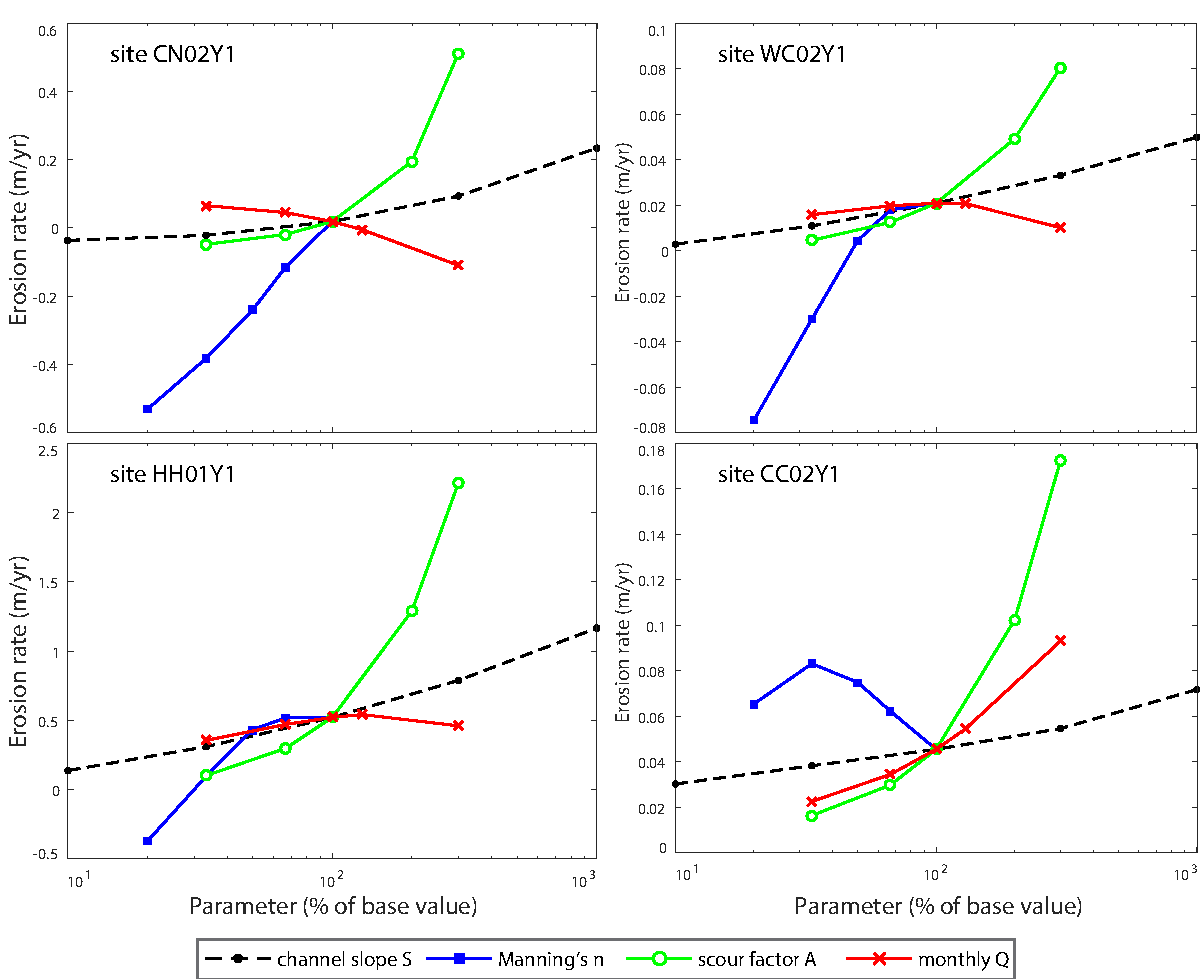
\includegraphics[width=6in]{figs/sensitivity.pdf}
\caption{Sensitivity of the modeled streambank erosion rates to 4 model parameters: channel slope $S$, Manning's $n$, scour factor $A$, average discharge $Q$. Changes in erosion rates resulting from changing each of these parameters independently are plotted for four study sites. The parameters are expressed as percentages of their base values discussed in the text.}\label{fig:sensitivity}
\end{figure}

\begin{figure}
\centering
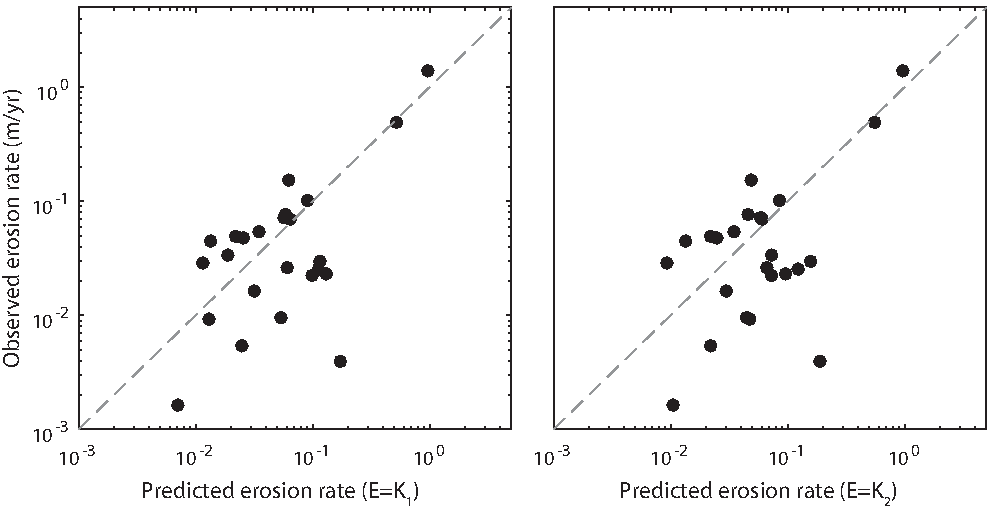
\includegraphics[width=1\textwidth]{figs/k1-vs-k2.pdf}
\caption[Results of model calibration]{Results of model calibration using soil erodibility parameters $K_1$ (\cref{eq:wynn}) and $K_2$ (\cref{eq:k2}). The model with $K_1$ predicts streambank erosion rates with a significant correlation ($R^2=0.91$, $p<0.001$, $\rho=0.53$). The model with $K_2$ predicts streambank erosion rates to a similar degree ($R^2=0.90$, $p<0.001$, $\rho=0.48$) but with fewer parameters. The dashed line is 1:1 correlation. Here, $R^2$ represents the square of the Pearson correlation coefficient $R$ between modeled and predicted erosion rates in their original units; $\rho$ is Spearman's rank correlation coefficient. See the text for discussion on interpreting these statistics for this dataset.} \label{fig:k1-vs-k2}
\end{figure}

\Cref{fig:hh01} shows the results of applying the model with $E=K_2$ to a medium-sized stream in a mixed pasture/forest landscape in Okaloosa County, FL. The simulation was run using the same input data used to train the model, including a monthly discharge time series of 24 mo. A few bends are currently meandering out of the riparian buffer zone into pastured areas, where tree cover is very low. High erosion rates of $>$0.75 m/yr were predicted on the non-forested section of the large bend downstream (south) of the calibration locations (HH01 and HH02), and rates of almost 1 m/yr were modeled on a tight, non-forested bend in southern part of the map. The non-forested bends all host erosion rates of well over 0.25 m/yr. Reasonably high erosion rates were not only confined to non-forested bends, however; several sharp bends in the forested portion of the image were predicted to erode up to 0.25 m/yr, comparable to the non-forested bend near HH01. The moderate erosion rates on these forested bends are associated with increased basal scour resulting from their high curvatures. Additionally, the upstream geometry of the meander train could have a cumulative downstream effect on erosion rates, as shown by G{\"u}neralp and Rhoads (\citeyear{Guneralp2009}, \citeyear{Guneralp2010}). The bottom panel plots channel curvature ($B/R$), velocity excess ($\Delta U/U$) and depth excess ($\Delta h/H$) against the downstream coordinate $s$ and shows the spatial lag between curvature and the velocity perturbations. \Cref{fig:hh01} illustrates the model's ability to predict streambank erosion rates throughout a 1 km reach displaying high variability in tree cover and channel geometry characteristics. 

\begin{figure}
\centering
\vspace{-1in}
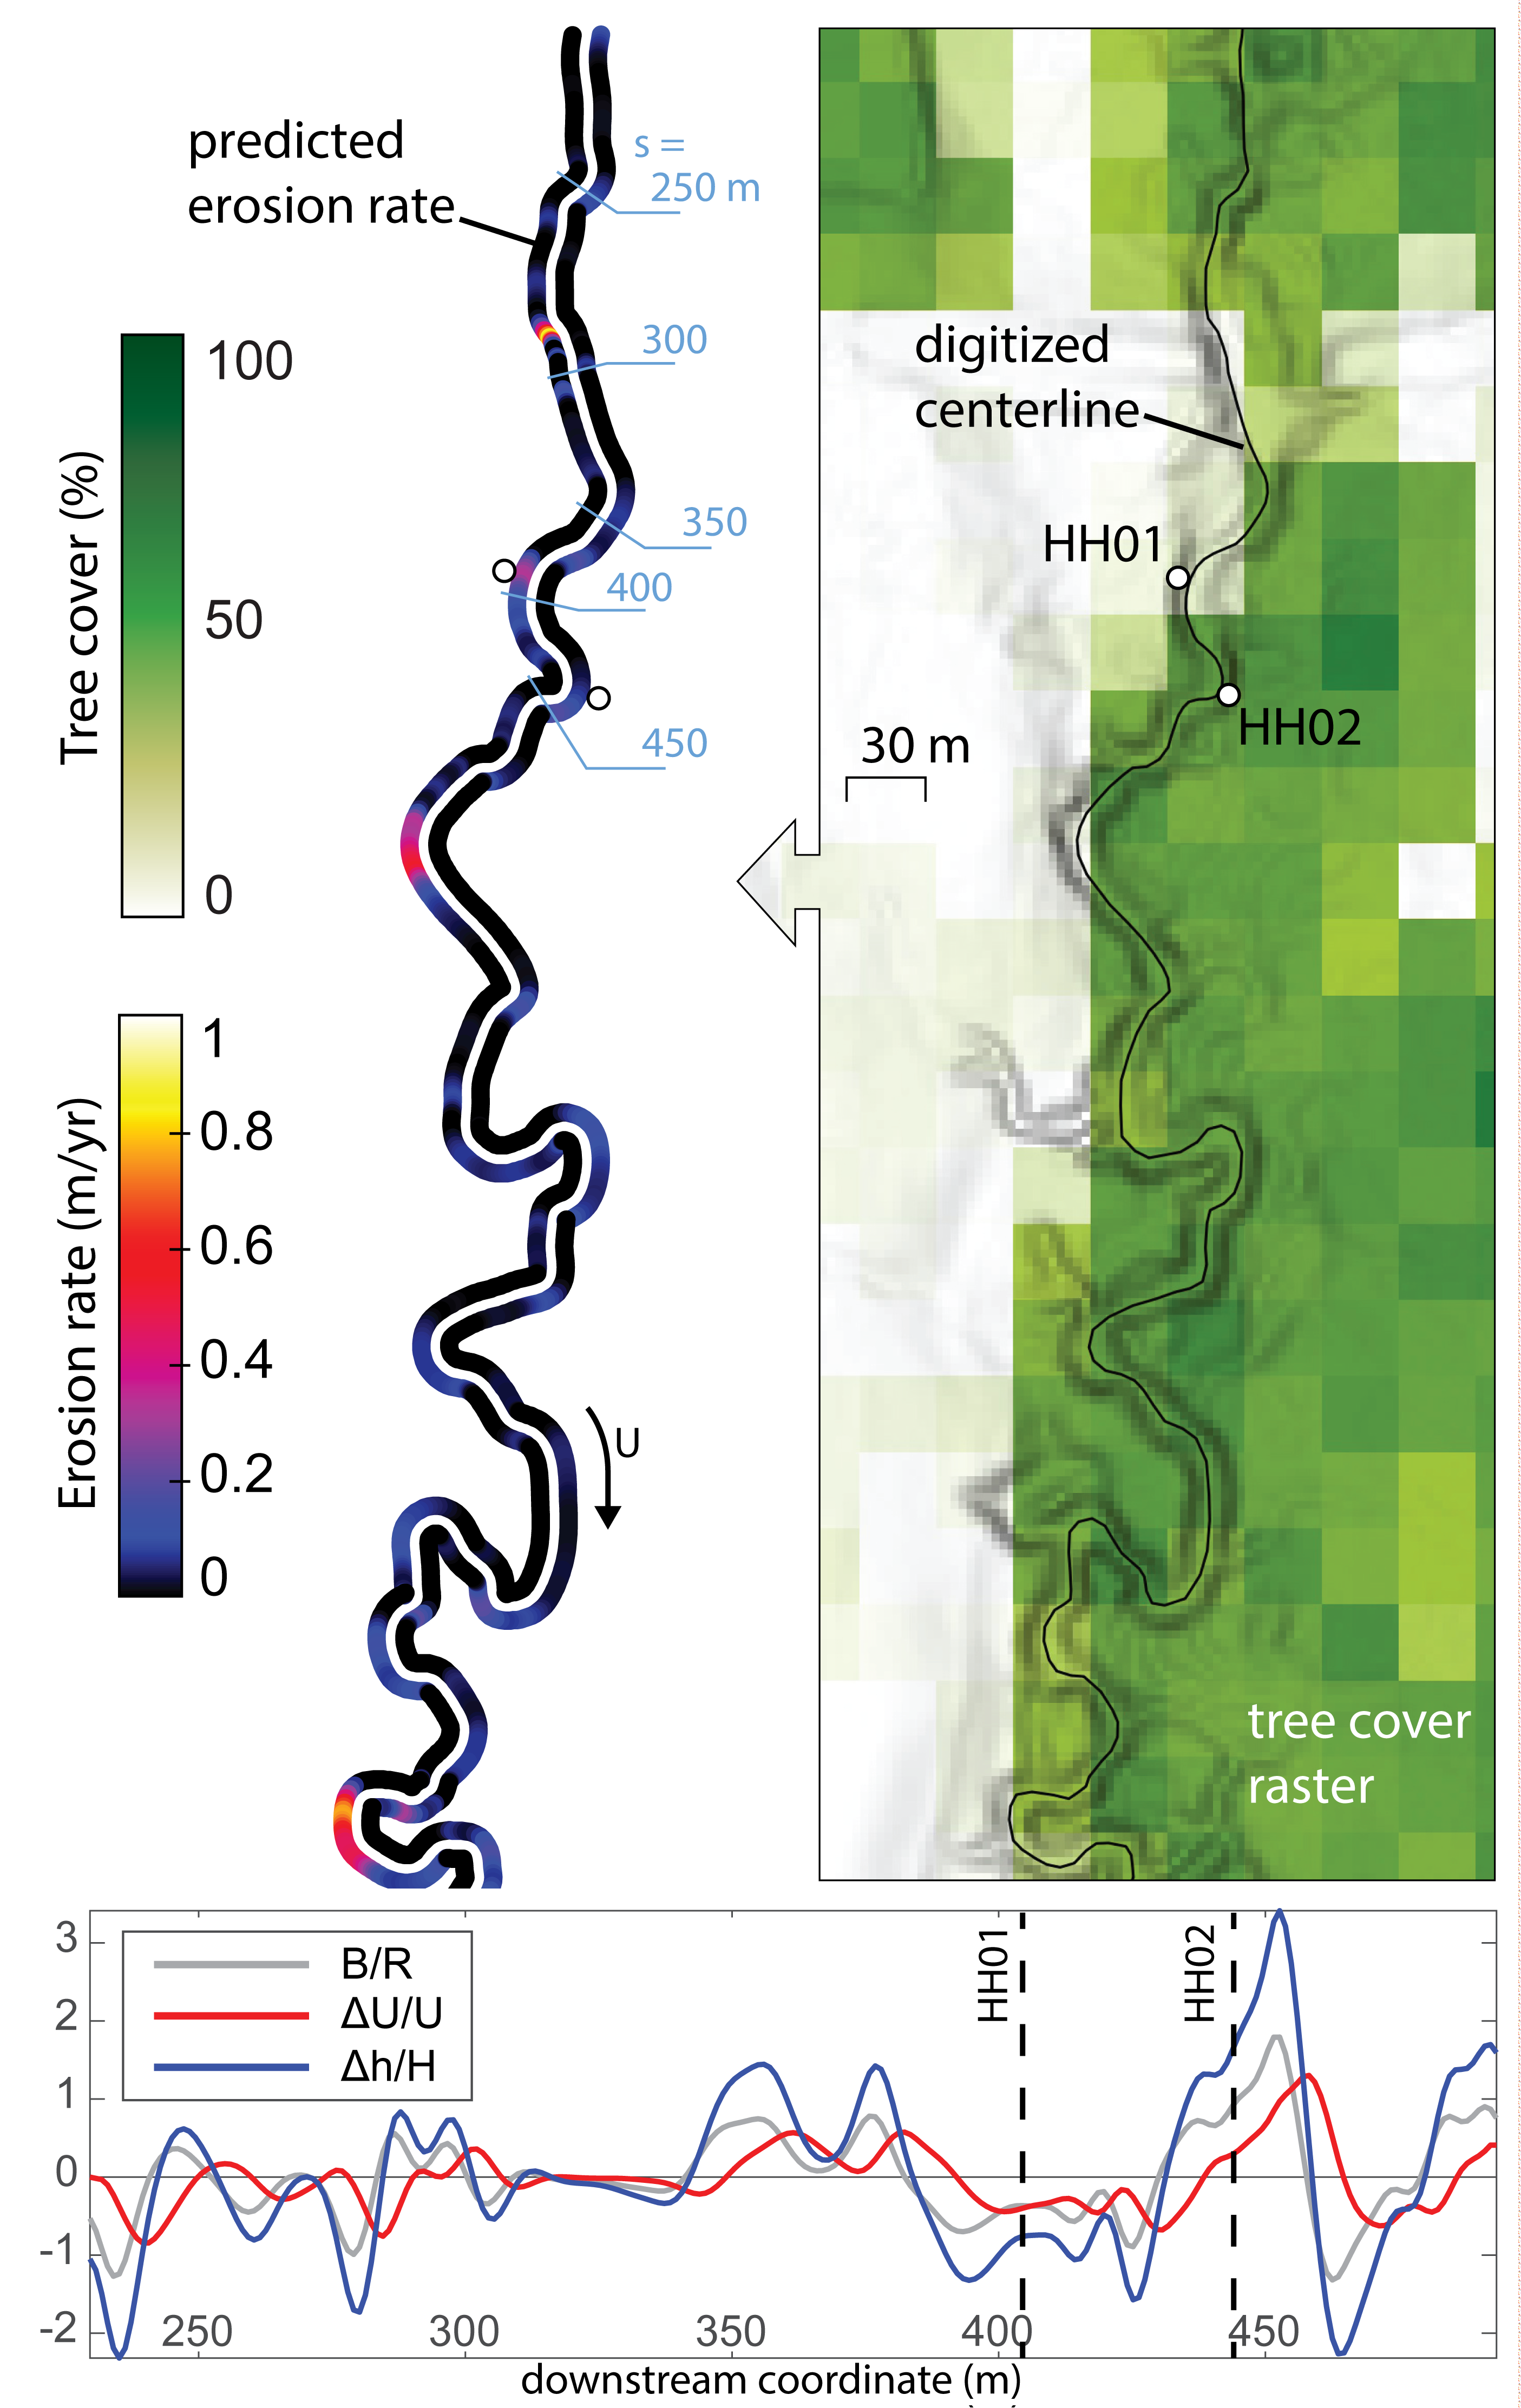
\includegraphics[width=0.8\textwidth]{figs/hh01-model-results.png}
\caption{Model application on Horsehead Creek (sites HH01 and HH02). Right: Input tree cover dataset (white to green) and channel centerline digitized on 3 m DEM (shown with slope shaded). Left: Modeled streambank erosion rates throughout the reach. Light blue numbers map the downstream coordinate plotted in the bottom panel. Flow is north to south. Bottom: Comparison of curvature ($B/R$), velocity excess ($\Delta U/U$), and depth excess ($\Delta h/H$) during the December 2015 simulation.}\label{fig:hh01}
\end{figure}

\section{Discussion}

We presented two models that predicted streambank erosion rates (\cref{fig:k1-vs-k2}). While both are highly correlated to observed erosion rates, the model incorporating $K_2$ for soil erodibility contains only three free parameters, while the model incorporating $K_1$ contains four. The negative relationship between bulk density and bank erosion reported by \citep{Wynn2006} was not observed here. This could be due to many factors. Soils with high organic matter and root biomass content would express lower bulk densities despite being less erodible overall, and sandy soils commonly express higher bulk densities as well as higher erodibility. The large-scale SSURGO dataset may also be unable to resolve the spatial heterogeneity of bank materials, especially for many of the small channels used to calibrate the model. This result agrees with recent work by \citet{Daly2015}, who found that watershed-scale relationships for bank erodibility based on soil properties showed no significant correlations to erodibility coefficient or critical shear stress. It is therefore not surprising that $K_1$ did not improve the bank erodibility estimation across the many watersheds of our study.

The overall effectiveness of $K_2$ agrees with the observations of \citet{Pizzuto1984}, \citet{Pizzuto1989}, and \citet{Pizzuto2010}, who found that forested streambank erodibility is largely controlled by tree density. Assuming representative values of tree cover of 5--10\% for pastured/agricultural areas and 40--60\% for forested areas, \cref{eq:k2res} predicts that forested streambanks retreat 4--12 times slower than non-forested ones. This generally agrees with previous studies, which have reported two to five-fold differences in bank erodibility between forested and non-forested streambanks (\citealp{Micheli2004}; \citealp{Allmendinger2005}; \citealp{Sass2012}). The relatively large (up to 12-fold) difference implied here is probably due to the extremely low erosion rates of forested streambanks in these low-gradient coastal plain streams, rather than especially high erosion rates of non-forested streambanks.

In both models, there appear to be two distinct groups of data points, one with largely positive residuals and another with negative residuals. Residuals were mapped and Moran's Index of $I=-0.09$ was calculated in \mbox{ArcMap}, indicating that the residuals are not spatially autocorrelated and are not statistically different from random ($p=0.86$). \Cref{fig:model-residuals} maps the residuals over Noah-2.8 surface runoff and PRISM precipitation totals for September 2015. Comparison to the PRISM data shows that some highly localized but intense storms were not represented well in the Noah-2.8 runoff simulations, either as a result of the coarse resolution of the NLDAS-2 forcing data, or because of inaccuracies in the Noah-2.8 LSM. Extreme rainfall totals and flash flooding were documented by weather stations in the area during this event (National Weather Service, North Central Gulf Coast Heavy Rain Event
27-29 September 2015, accessed 16 June 2016, \url{https://www.weather.gov/mob/heavyrain_sep2015}). It is likely that the Noah-2.8 underestimated surface runoff during such small intense storms, which may have contributed to the negative residuals shown on the map (\cref{fig:model-residuals}).

\begin{figure}
\centering
\frame{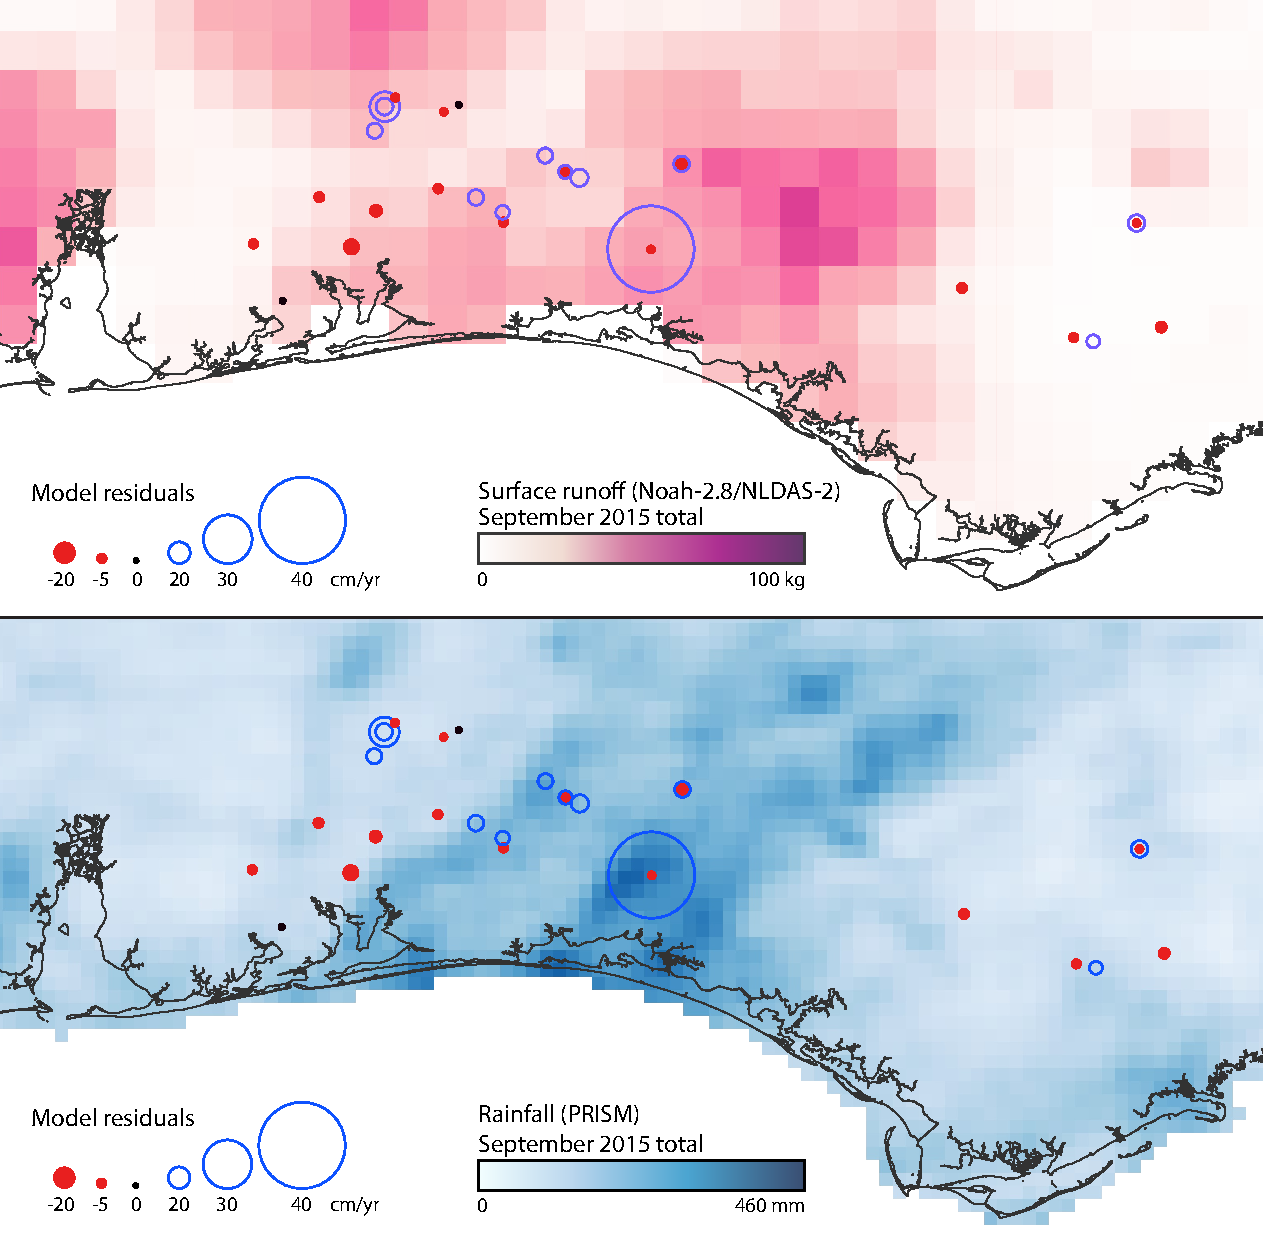
\includegraphics[width=1\textwidth]{figs/model-residuals.pdf}}
\caption{Map of residuals. Comparison of Noah-2.8 surface runoff (top) and PRISM precipitation (bottom) for September 2015 demonstrates discrepancies in the Noah model. A small but intense storm near the middle of the map is not represented in the surface runoff data.} \label{fig:model-residuals}
\end{figure}

It would be useful to compare the model of this paper to similar models in the literature, but few if any comparable models exist. We therefore fit two simple models for comparison: a purely empirical statistical model and an Ikeda-type model based on \cref{eq:equation} with a spatially constant erodibility coefficient $E$. All models were fit using the nonlinear regression procedure outlined in \cref{sec:regression}. \Cref{tab:compare} shows that the model of this paper, using either $K_1$ or $K_2$, outperforms these simpler models according to Spearman's rank correlation coefficient $\rho$, which is robust to outliers. $R^2$ is reported as the square of the correlation coefficient between the predicted and actual streambank erosion rates, but is skewed by outliers. The negative exponents on slope and drainage area exhibited by the purely empirical model are likely not physically sound, and $\rho<0$ indicates an overall negative relationship to erosion rates. The Ikeda-type model is positively correlated to erosion rates, but this correlation is not as strong as the models proposed here. This comparison illustrates the utility of combining the BdV hydrodynamic model with a spatially distributed bank erodibility relationship. 

\begin{table}
\centering
\begin{tabular}{lll}
\toprule
Model & Description & Statistics\\
\midrule
\cref{eq:k1res} & This paper, $K_1$ & $R^2=0.91$, $\rho=0.53$\\
\cref{eq:k2res} & This paper, $K_2$ & $R^2=0.90$, $\rho=0.48$\\
$\hat{\zeta} = 0.032\mathit{BD}^{-5.4}S^{-0.037}A^{-0.86}\mathit{TC}^{-2.8}$ & Empirical model & $R^2=0.98$, $\rho=-0.20$\\
$\hat{\zeta} = 1.54 \overline{\Delta U}$ & \cref{eq:equation} & $R^2=0.034$, $\rho=0.25$\\
\bottomrule
\end{tabular}
\caption{Comparison of the model of this paper with a purely empirical model and a model lacking spatial variability in bank erodibility (an Ikeda-type model based on \cref{eq:ikeda}).}\label{tab:compare}
\end{table}

An existing spatially distributed model for total sediment yield from drainage basins, SedNet, quantifies annual streambank erosion as a function of bankfull stream power, bank erodibility, and a daily streamflow factor (\citealp{Wilkinson2009}, \citeyear{Wilkinson2014}). The SedNet model requires a long-term dataset of daily streamflow observations as well as two raster datasets: one representing vegetation cover (values of 0 to 1, with 1 representing fully intact riparian vegetation) and another of bank erodibility (values of 0 or 1, with 0 representing bedrock and 1 representing pixels characterized as soil). Rather than modelling the spatial variability introduced by hydrodynamic processes, SedNet models the average bank erosion of entire stream links. SedNet was not designed to allow the prediction of local streambank erosion rates, or the identification of erosion hot-spots, but rather to simulate the large-scale processes exporting sediment from large drainage basins; streambank erosion is just one part of the model. Nevertheless, it is increasingly being used to estimate local streambank erosion rates because it is the only spatially distributed model that attempts to do so \citep{Bartley2008}. One recent evaluation of the accuracy of the streambank erosion rates predicted by SedNet showed that its original predictions differed from measured erosion rates (averaged over 10 locations) by a factor of 74, but this discrepancy was decreased to a factor of $\sim$2 with calibration to field-measured values of bed slope and bankfull discharge.

The main goal of this paper was to develop a spatially distributed model that incorporated widely available data and could be readily used in practical applications. This approach necessitated a few simplifications. Meander migration models based on \Cref{eq:ikeda} usually assume some a constant discharge to determine $\Delta U$, e.g., mean annual $Q$, bankfull $Q$, or another statistic \citep{Camporeale2010}. Here, we computed a monthly-varying discharge statistic $Q*$, and ran the BdV model on this timestep before averaging the monthly estimates of $\Delta U$. This approach was designed to account for variability in precipitation and runoff at the regional scale, and for increased erosion during high flow periods. This is a novel application of \cref{eq:ikeda}, however, and it has not been shown that streambank erosion rates are proportional to $\Delta U$ on these shorter timescales.

The sensitivity analysis showed that the model is sensitive to errors in Manning's roughness coefficient $n$ and the scour factor $A$, but these parameters are difficult to estimate using only remotely sensed data, or other widely available datasets. We assumed characteristic values for these parameters and held them constant throughout the study area. This is a major limitation of the model and likely a source of error. In the future, reach-scale measurements of $n$ and $A$ should be incorporated into the model.

Another limitation of the model is its reliance on an \emph{ad hoc} method for determining the relevant monthly discharge, which was estimated as a function of average monthly discharge and storm frequency. The lack of streamgages in the basins being studied necessitated modelling of monthly streamflow. The average monthly streamflow estimates are from the Noah-2.8 LSM, a large-scale land surface model designed to simulate processes acting at the global, continental, and large watershed scale. Such models have been shown to be relatively inaccurate at predicting streamflow in small basins, though they often express a higher skill in the southeastern U.S. than in other regions \citep{Xia2012}.

A thorough validation of this model is outside the scope of this paper, but should be done at the reach and watershed scales. The model could be evaluated on a few reaches where channel geometry is known or can be easily measured. Existing streambank erosion rate databases could be useful for model validation, provided that the GPS coordinates of streambank measurements can be determined accurately.

\section{Conclusions}

\citet{Bartley2008} remarked that ``it will be difficult for catchment scale sediment budget models to ever accurately predict the location and rate of bank erosion due to the variation in bank erosion rates in both space and time.'' \citet{DeVente2013} cited the lack of a bank erosion component as a major limitation of current sediment detachment models. We presented a spatially distributed model for streambank erosion incorporating an empirical soil erodibility parameter ($K_2$), a nonlinear hydrodynamic model, and monthly discharge forcings. An application of the model to a medium-sized stream in the Gulf Coastal plain (\cref{fig:hh01}) demonstrated its potential for quantifying annual streambank erosion throughout a mixed forest/pasture reach. Although future work should focus on improving the model's parameterization of roughness and streamflow, as well as a thorough evaluation and validation of model predictions throughout multiple reaches, the current model shows a significant correlation to observed erosion rates. The model thus represents a first step toward filling the long-standing gap emphasized by \citet{Bartley2008} and \citet{DeVente2013}. 

\section{Acknowledgments}
We thank David Cambron and Michele Goodfellow for their help in collecting data for this study. This study was based on work supported by a grant from the Florida Fish and Wildlife Conservation Commission and the U.S. Fish and Wildlife Service (State Wildlife Grant 13058). The Geological Society of America, the Gulf Coast Association of Geological Societies, and the University of West Florida Scholarly and Creative Activities Committee provided additional funding. The authors thank Dr. Jim Pizzuto and an anonymous reviewer for their thoughtful critique of this paper. The paper was greatly improved by their comments.

\bibliographystyle{elsarticle-harv-EDITED} 
\bibliography{sublibrary}

\end{document}
\endinput

